%definira klasu dokumenta 
\documentclass[12pt]{report} 

%prostor izmedu naredbi \documentclass i \begin{document} se zove uvod. U njemu se nalaze naredbe koje se odnose na cijeli dokument

%osnovni LaTex ne može riješiti sve probleme, pa se koriste različiti paketi koji olakšavaju izradu željenog dokumenta
\usepackage{listings}
\usepackage[croatian]{babel} 
\usepackage{amssymb}
\usepackage{amsmath}
\usepackage{txfonts}
\usepackage{mathdots}
\usepackage{titlesec}
\usepackage{array}
\usepackage{lastpage}
\usepackage{etoolbox}
\usepackage{tabularray}
\usepackage{color, colortbl}
\usepackage{adjustbox}
\usepackage{geometry}
\usepackage[classicReIm]{kpfonts}
\usepackage{hyperref}
\usepackage{fancyhdr}
\usepackage{comment}

\usepackage{float}
\usepackage{setspace}
\restylefloat{table}


\patchcmd{\chapter}{\thispagestyle{plain}}{\thispagestyle{fancy}}{}{} %redefiniranje stila stranice u paketu fancyhdr

%oblik naslova poglavlja
\titleformat{\chapter}{\normalfont\huge\bfseries}{\thechapter.}{20pt}{\Huge}
\titlespacing{\chapter}{0pt}{0pt}{40pt}


\linespread{1.3} %razmak između redaka

\geometry{a4paper, left=1in, top=1in,}  %oblik stranice

\hypersetup{ colorlinks, citecolor=black, filecolor=black, linkcolor=black,	urlcolor=black }   %izgled poveznice


%prored smanjen između redaka u nabrajanjima i popisima
\newenvironment{packed_enum}{
	\begin{enumerate}
		\setlength{\itemsep}{0pt}
		\setlength{\parskip}{0pt}
		\setlength{\parsep}{0pt}
	}{\end{enumerate}}

\newenvironment{packed_item}{
	\begin{itemize}
		\setlength{\itemsep}{0pt}
		\setlength{\parskip}{0pt}
		\setlength{\parsep}{0pt}
	}{\end{itemize}}




%boja za privatni i udaljeni kljuc u tablicama
\definecolor{LightBlue}{rgb}{0.9,0.9,1}
\definecolor{LightGreen}{rgb}{0.9,1,0.9}

%Promjena teksta za dugačke tablice
\DefTblrTemplate{contfoot-text}{normal}{Nastavljeno na idućoj stranici}
\SetTblrTemplate{contfoot-text}{normal}
\DefTblrTemplate{conthead-text}{normal}{(Nastavljeno)}
\SetTblrTemplate{conthead-text}{normal}
\DefTblrTemplate{middlehead,lasthead}{normal}{Nastavljeno od prethodne stranice}
\SetTblrTemplate{middlehead,lasthead}{normal}

%podesavanje zaglavlja i podnožja

\pagestyle{fancy}
\lhead{Programsko inženjerstvo}
\rhead{Projektni zadatak}
\lfoot{Jarci\&Magarci}
\cfoot{stranica \thepage/\pageref{LastPage}}
\rfoot{\today}
\renewcommand{\headrulewidth}{0.2pt}
\renewcommand{\footrulewidth}{0.2pt}


\begin{document} 
	
	
	
	\begin{titlepage}
		\begin{center}
			\vspace*{\stretch{1.0}} %u kombinaciji s ostalim \vspace naredbama definira razmak između redaka teksta
			\LARGE Programsko inženjerstvo\\
			\large Ak. god. 2021./2022.\\
			
			\vspace*{\stretch{3.0}}
			
			\huge Inventura\\
			\Large Dokumentacija, Rev. \textit{1}\\
			
			\vspace*{\stretch{12.0}}
			\normalsize
			Grupa: \textit{Jarci\&Magarci}\\
			Voditelj: \textit{Elena Wachtler}\\
			
			
			\vspace*{\stretch{1.0}}
			Datum predaje: \textit{$19$. $11$. $2021$.}\\
	
			\vspace*{\stretch{4.0}}
			
			Nastavnik: \textit{Igor Stančin, mag. ing.}\\
		
		\end{center}

	
	\end{titlepage}

	
	\tableofcontents


	\chapter{Dnevnik promjena dokumentacije}
		
		\textbf{\textit{Kontinuirano osvježavanje}}\\
				
		
		\begin{longtblr}[
				label=none
			]{
				width = \textwidth, 
				colspec={|X[2]|X[13]|X[3]|X[3]|}, 
				rowhead = 1
			}
			\hline
			\textbf{Rev.}	& \textbf{Opis promjene/dodatka} & \textbf{Autori} & \textbf{Datum}\\[3pt] \hline
			0.1 & Napravljen predložak.	& Filip Begović & 26.10.2021. 		\\[3pt] \hline 
			0.2 & Dodan opis projektnog zadataka i funkcionalni zahtjevi. & Nina Anić, Filip Begović, Marko Bagarić & 26.10.2021. \\[3pt] \hline
			0.3 & Napravljeni obrasci uporabe. & Nina Anić, Filip Begović & 2.11.2021.\\[3pt] \hline
			0.4 & Dijagrami obrazaca uporebe, sekvencijski dijagram i ostali zahtjevi & Filip Begović, Tin Jukić & 10.11.2021. 13.1.2022. \\[3pt]\hline
			0.4	& Unos sličnih aplikacija & Marko Bagarić & 27.10.2021. 	\\[3pt] \hline 
			0.5 & Dodan \textit{Use Case} dijagram i jedan sekvencijski dijagram, funkcionalni i nefunkcionalni zahtjevi i dodatak A & Filip Begović &  15.11.2021. \\[3pt] \hline 
			0.6 & Inicijalni dizajn ekrana aplikacije & Filip Begović & 28.10.2021. \\[3pt] \hline 
			0.9 & Opisi obrazaca uporabe & Filip Begović & 15.11.2021. \\[3pt] \hline 
			0.10 & ER dijagram i opis tablice baze podataka & Elena Wachtler & 18.11.2021. \\[3pt] \hline 
			0.11 & Sekvencijski dijagrami & Filip Begović & 15.11.2021. \\[3pt] \hline 
			0.12.1 & Dijagrami razreda & Tin Jukić & 15.11.2021. 12.1.2022. \\[3pt] \hline 
			0.12.2 & Dovršen dio dokumentacije Arhitektura i dizajn sustava & Tin Jukić & 12.1.2022. \\[3pt] \hline 
			\textbf{1.0} & Verzija samo s bitnim dijelovima za 1. ciklus & Elena Wachtler, Tin Jukić, Filip Begović & 18.11.2021. \\[3pt] \hline 
			1.1 & Ostali dijagrami iz Arhitekture & Tin Jukić & 12.1.2022. \\[3pt] \hline 
			1.2 & Korištene tehnologije i alati & Marko Bagarić & 13.1.2022. \\[3pt] \hline 
			1.5 & Ispitivanje programskog rješenja & Marko Bagarić & 13.1.2022. \\[3pt] \hline 
			1.5.1 & Dijagram razmještaja & Marko Bagarić, Borna Rebić-Taučer & 13.1.2022. \\[3pt] \hline 
			1.5.2 & Upute za puštanje aplikacije u pogon & Borna Rebić-Taučer & 13.1.2022. \\[3pt] \hline
			\textbf{2.0} & Konačni tekst predloška dokumentacije  & * & 13.1.2022. \\[3pt] \hline 
			&  &  & \\[3pt] \hline	
		\end{longtblr}
	
		\begin{comment}
		\textit{Moraju postojati glavne revizije dokumenata 1.0 i 2.0 na kraju prvog i drugog ciklusa. Između tih revizija mogu postojati manje revizije već prema tome kako se dokument bude nadopunjavao. Očekuje se da nakon svake značajnije promjene (dodatka, izmjene, uklanjanja dijelova teksta i popratnih grafičkih sadržaja) dokumenta se to zabilježi kao revizija. Npr., revizije unutar prvog ciklusa će imati oznake 0.1, 0.2, …, 0.9, 0.10, 0.11.. sve do konačne revizije prvog ciklusa 1.0. U drugom ciklusu se nastavlja s revizijama 1.1, 1.2, itd.}
		\end{comment}
	\chapter{Opis projektnog zadatka}
		
		Cilj ovog projekta je izrada mobilne aplikacije „Inventura“ koja će korisniku olakšati posao inventure skladišta. Tvrtke čiji zaposlenici će koristiti ovu aplikaciju imaju nekoliko skladišta na različitim lokacijama te će pomoću ove aplikacije i mobilne kamare moći očitati bar kodove i QR kodove artikala čiju inventuru žele napraviti. Također, ovisno o tome koju ulogu u tvrtci korisnik ima, aplikacija mu nudi određene funkcionalnosti kao što su: prikaz informacija o artiklu, njegova lokacija, broj artikala, mogućnost povećanja i smanjenja broja artikala, spremanje promjena u bazu, slanje obavijesti nadležnima, kontrola inventure, preraspodjela artikala po grupama i mnoge druge.
		
		Prilikom pokretanja aplikacije korisniku se prikazuje stranica za prijavu registriranih korisnika na kojoj se nalaze polja za unos email adrese i lozinke. Neregistrirani korisnik pri dnu stranice za prijavu treba odabrati opciju „Registriraj se“ koja ga vodi na stranicu za registraciju. Za kreiranje novog računa potrebno je navesti:
		
		\begin{packed_item}
			\item \textit{Ime}
			\item \textit{Prezime}
			\item \textit{Email}
			\item \textit{Lozinku}
			\item \textit{Ulogu u tvrtci}
			\item \textit{Ovisno o ulozi u tvrtci, skladište u kojem zaposlenik radi}
		\end{packed_item}
	
		Kada se korisnik prijavi u sustav uključuje mu se stražnja kamera mobilnog uređaja te se prikazuje početni zaslon koji je spreman za očitavanje bar koda i QR koda. Osim što može očitati kodove, korisnik ovisno o svojoj ulozi ima još dodatnih mogućnosti.
		
		\underbar{Korisnik može imati jednu od ove tri uloge:}
		\begin{packed_item}
			\item \textit{Skladištar}
			\item \textit{Šef skladišta}
			\item \textit{Direktor}
		\end{packed_item}
	
		\underbar{Skladištar} je osoba koja obavlja inventuru skladišta te po potrebi obavještava svoje nadležne ako određenog artikla nema na skladištu. Biranje artikla za skeniranje se vrši automatski, na način da prvi artikl koji skenira u toj inventuri je onaj odabrani. Zatim se uključi stražnja kamera mobilnog uređaja te se na ekranu aplikacije prikazuje početni zaslon koji je spreman za skeniranje. Kada se na proizvodu skenira te mu se detektira bar kod ili QR kod, skladištaru na zaslonu aplikacije iskače prozor (engl.\emph{pop-up window}) koji se prikazuje 5 sekundi. Taj prozor sadrži informacije o skeniranom proizvodu u obliku kratkog opisa, lokaciju na kojoj je skeniran (dohvaćenu automatski pomoću GPS modula mobitela) i brojač takvih proizvoda u skladištu, a također i nudi opcije povećanja i smanjenja broja proizvoda, odbacivanje trenutnog očitanja bez spremanja u bazu, te pohranu trenutnog očitanja u bazu bez čekanja da istekne 5 sekundi. Promjenom broja očitanih artikala resetira se brojač 5 sekundi, a istekom vremena brojača zapis se automatski sprema u bazu. Na početnom zaslonu postoji i opcija \emph{Završi}. Odabirom te opcije skladištar završava svoj rad nad tim proizvodom. Svaki skladištar može skenirati samo jednu vrstu proizvoda dok ne označi završetak skeniranja tog proizvoda. Osim opcije za skeniranje proizvoda, skladištaru se na početnoj stranici nudi još i mogućnost odjave iz aplikacije te povijest svih unosa proizvoda. Odabirom prikaza povijesti, sustav korisniku prikazuje pregled povijesti svih unosa korisnika. Prvo prema odrađenim inventurama, uz koje se prikazuje datum inventure. Pritiskom na izabranu inventuru prikazuju se svi proizvodi koje je prijavljeni skladištar unio u aplikaciju, dok pritiskom na još aktivnu inventuru, uza sve unesene proizvode skladištar može dojaviti šefu skladišta da nekog artikla nema na skladištu. Prilikom pregleda povijesti unosa, za svaki artikl navodi se njegov naziv, lokacija na kojoj je skeniran te broj koliko je takvih artikala prijavljeni skladištar skenirao.
		
		\underbar{Šef skladišta}, za razliku od ostalih korisnika, ima mogućnost korištenja aplikacije na 1 od 2 načina: kao izvršitelj inventure ili kao kontrolor inventure. Prilikom ulaska u aplikaciju otvara mu se kamera za detekciju bar kodova i QR kodova. Ukoliko je skenirao proizvod koji u trenutnoj inventuri nije bio skeniran tada ima ulogu izvršitelja inventure. Za razliku od toga, ako je proizvod već skeniran u trenutnoj inventuri, tada ima ulogu kontrolora inventure.\\Kao izvršitelj inventure, dobiva jednaku funkcionalnost kao i skladištar i uključuje mu se kamera mobilnog uređaja. Zatim se na ekranu aplikacije prikazuje početni zaslon koji je spreman za skeniranje. Kada se proizvodu skenira i detektira bar kod ili QR kod, šefu skladišta na zaslonu aplikacije iskače prozor (engl. \emph{pop-up window}) koji se prikazuje 5 sekundi. Taj prozor sadrži informacije o skeniranom proizvodu, lokaciju na kojoj je skeniran (automatsko dohvaćanje pomoću GPS modula mobitela) i brojač takvih proizvoda u skladištu te nudi opcije povećanja i smanjenja broja proizvoda, odbacivanje trenutnog očitanja bez spremanja u bazu te pohranu trenutnog očitanja u bazu bez čekanja da istekne 5 sekundi. Promjenom broja očitanih artikala resetira se brojač 5 sekundi, a istekom vremena brojača zapis se automatski sprema u bazu. Na početnom zaslonu postoji i opcija \emph{Završi}. Odabirom te opcije označava se završetak skeniranja odabranog artikla. Osim opcije za skeniranje proizvoda, šefu skladišta se nude još četiri mogućosti na početnom zaslonu: pregled svih artikala na skladištu, pregled svih izvršenih inventura nad tim skladištem, pregled obavijesti te izlazak (odjava) iz aplikacije. Odabirom prikaza povijest prikazuje se pregled povijesti svih unosa korisnika. Prvo prema odrađenim inventurama, uz koje se prikazuje datum inventure. Odabirom određene inventure, šefu skladišta se nudi opcija pregleda svih artikala na skladištu tako da se za svaki artikl ispisuje njegov naziv, lokacija te broj takvih artikala na skladištu. Odabirom prikaza pošte na početnom zaslonu, šefu skladišta se otvara stranica s obavijestima. Navedene obavijesti poslali su skladištari koji su uočili da određenih artikala nema na skladištu. Odabirom opcije prikaza svih proizvoda, šef skladišta može vidjeti sve artikle koji se trenutno nalaze na njegovom skladištu.\\Kao kontrolor inventure šef skladišta ima iste funkcionalnosti kao i skladištari. Jedina razlika je što odabirom opcije \emph{Završi}, ukoliko je broj skeniranih artikala od strane šefa skladišta različit od broja koje je skenirao skladištar, aplikacija automatski o tome obavještava direktora.
		
		\underbar{Direktor tvrtke} je korisnik aplikacije kojem su omogućene najveće funkcionalnosti i koji ima pristup gotovo svim do sad navedenim mogućnostima. Naime, nakon prijave u sustav otvara mu se početni zaslon i uključuje stražnja kamera mobilnog uređaja kako bi mogao skenirati artikl. Kada se proizvodu skenira i detektira bar kod ili QR kod, direktoru na zaslonu aplikacije iskače prozor (engl. \emph{pop-up window}) koji se prikazuje 5 sekundi. Taj prozor sadrži informacije o skeniranom proizvodu, lokaciju na kojoj je skeniran (automatsko dohvaćanje pomoću GPS modula mobitela) i brojač takvih proizvoda u skladištu te nudi opcije povećanja i smanjenja broja proizvoda, odbacivanje trenutnog očitanja bez spremanja u bazu te pohranu trenutnog očitanja u bazu bez čekanja da istekne 5 sekundi. Promjenom broja očitanih artikala resetira se brojač 5 sekundi, a istekom vremena brojača zapis se automatski sprema u bazu. Na zaslonu postoji i opcija \emph{Završi sken} čijim se odabirom završava rad nad tim artiklom, kao i opcija \emph{Završi inventuru} čijim se odabirom završava trenutna inventura te automatski počinje nova. Osim opcije za skeniranje proizvoda, direktoru tvrtke nude se još tri mogućnosti na početnom zaslonu: pregled svih skladišta u kojima se obavljala inventura, pregled obavijesti te izlazak (odjava) iz aplikacije. Odabirom svih inventura direktoru se nudi opcija pregleda svih skladišta u kojima se obavljala inventura. Nakon što direktor odabere određeno skladište, otvara mu se nova stranica na kojoj može odabrati želi li pretraživati skladištare koji su obavljali inventure ili artikle koji su bili skenirani. Ako odabere opciju \emph{Artikli} prikazuju mu se svi skenirani artikli u tom skladištu, te za svaki artikl njegovo ime i broj takvih artikala u odabranom skladištu. Osim što ima uvid u postojeće artikle, odabirom dodavanja novih kategorija direktoru se nudi opcija dodavanja grupa proizvoda i preraspodjela artikala po grupama. Za te funkcionalnosti otvara mu se nova stranica u kojoj može dodati novu grupu proizvoda, otići na već postojeću grupu ili preraspodijeliti artikle po grupama. Grupe proizvoda su organizirane u stablo s korijenom „proizvod“, a dubina i širina stabla nisu ograničeni. Osim opcije \emph{Artikli} postoji i opcija \emph{Skladištari} koja direktoru tvrtke prikazuje ime skladištara koji je radio inventuru u odabranom skladištu te njegovu statistiku pogreške. Odabirom popisa skladišta, prikazuje se ponovno popis svih skladišta, ali pritiskom na jedno od skladišta otvara se nova stranica s popisom svih inventura na tom skladištu. Odabirom određene inventure, direktor ima uvid u sve proizvode koji su se skenirali u toj inventuri. Odabirom opcije pregleda obavijesti, direktoru tvrtke otvara se stranica s obavijestima koje su poslali šefovi skladišta. Navedene obavijesti direktor može označiti odabirom odgovarajuće opcije kao riješene ili kao odbačene. Također, direktor ima pristup povijesti svih obavijesti.\\
		
		\large{\textbf{\textit{Postojeća slična rješenja}}}\normalsize
		
		\underbar{\textbf{1. EZOfficeInventory}}
		
		Jedna od popularnih aplikacija za vođenje inventure je EZOfficeInventory, aplikacija koja na bazi QR koda i bar koda omogućava skeniranje i praćenje inventure. Uz samo skeniranje kodova pomoću aplikacije, omogućuje povezivanje i RIFD čitača za olakšanu primjenu. Kako bi se lakše pratili proizvodi unutar skladišta omogućeno je i praćenje statistike podjeljive na više lokacija, timova itd., te podjelu ljudi po ulogama unutar same firme.
		
		\begin{figure}[H]
			
\includegraphics[height=5cm]{slike/EZ_logo.png}
			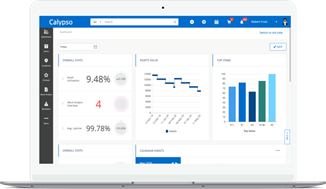
\includegraphics[height=5cm]{slike/EZ_slika.png}
			\centering
			\label{ez_logo}
		\end{figure}
		
		\underbar{\textbf{2. CountIt - Inventory application}}
		
		CountIt omogućava povezivanje više mobilnih uređaja na više lokacija skladišta te sve promjene sprema na oblak. Praćenje broja uživo, skeniranje podataka i spremanje uživo na oblak. Uz to, aplikacija omogućuje i dodjelu poslova, statistike praćenja cijele inventure te prilično fleksibilan plan korištenja, jeftiniji od ostalih konkurenata te se može bilo kada otkazati (za veće grupe i više opcija skuplje).
		
		\begin{figure}[H]
			
\includegraphics[height=5cm]{slike/CT_logo.png}
			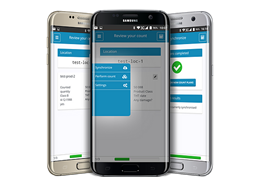
\includegraphics[height=5cm]{slike/CT_slika.png}
			\centering
			\label{ct_logo}
		\end{figure}
		
		\underbar{\textbf{3. Erply: Stocktake app}}
		
		Erply, uz dosadašnje implementacije različitih funkcija, nudi i offline brojanje artikla (prilikom spremanja u bazu naravno ponovno mora ići online ili prebaciti podatke na računalo kablom), pomoću povijesti skeniranih kodova nudi brže prepoznavanje i samo skeniranje, notifikacije korisnicima ukoliko se broj proizvoda previše smanji.
		
		\begin{figure}[H]
			
\includegraphics[height=5cm]{slike/ER_logo.png}
			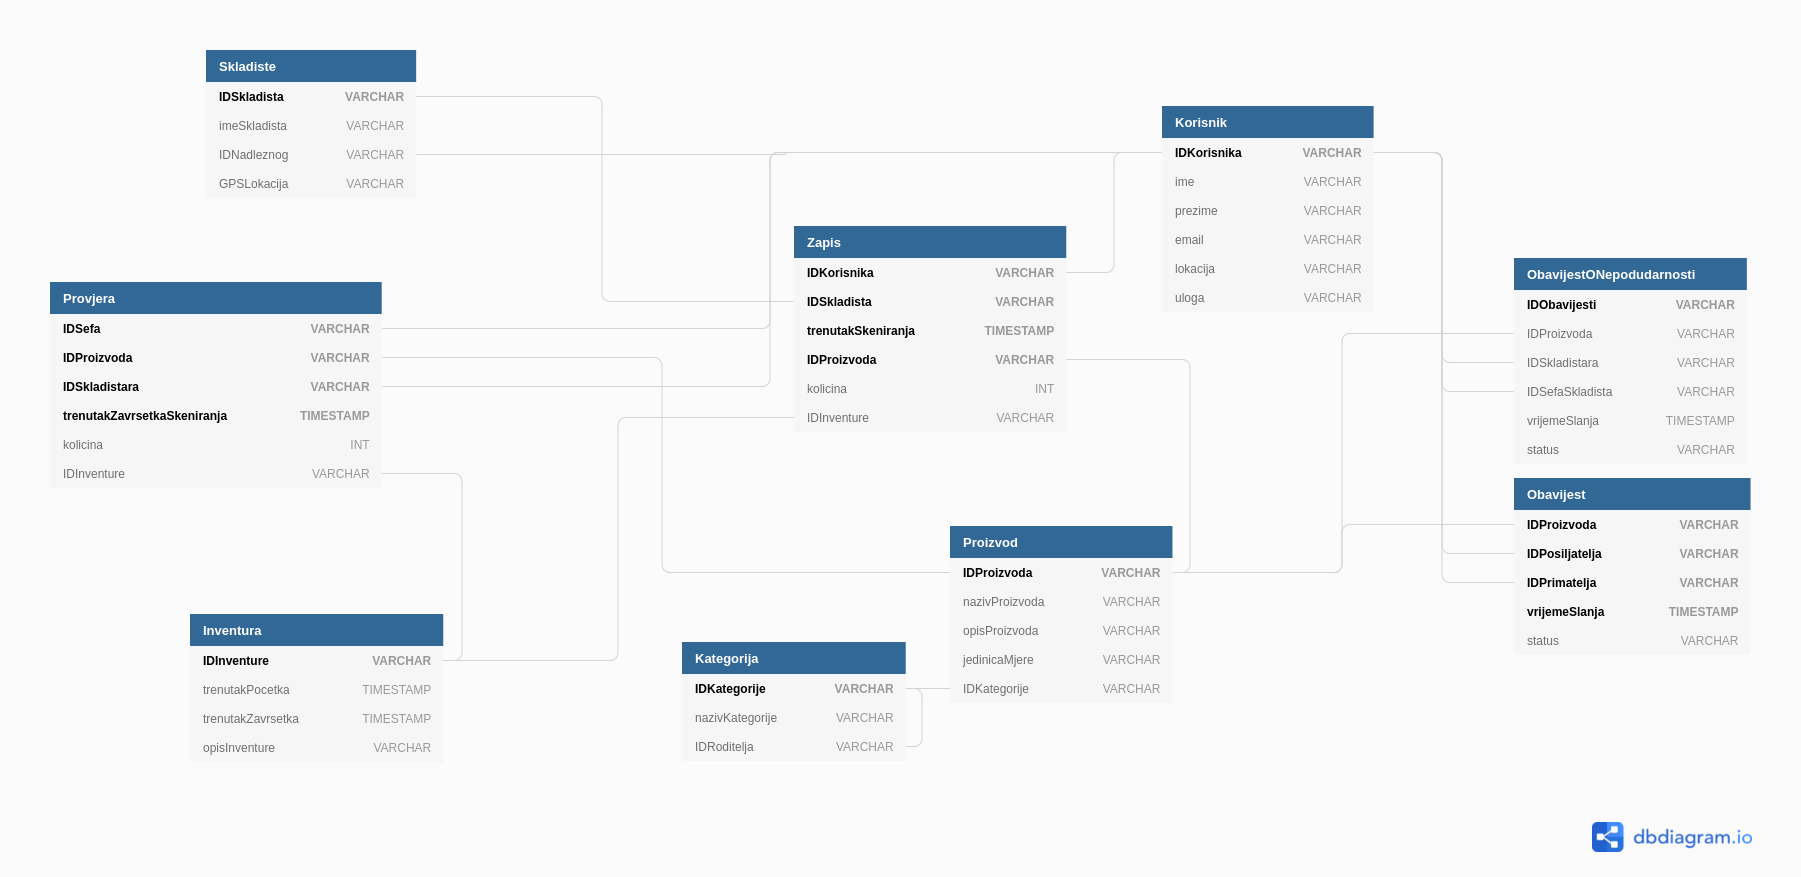
\includegraphics[height=5cm]{slike/ER_slika.png}
			\centering
			\label{er_logo}
		\end{figure}
		
		\underbar{\textbf{4. Stockpile by Canvus}}
		
		Besplatna i jednostavnija verzija dosadašnjih aplikacija koja se fokusira na manje privatne firme kako bi im olakšali provođenje inventure. Aplikacija, za razliku od ostalih, ne nudi skeniranje kodova proizvoda, ali sadrži osnovne funkcionalnosti potrebne za provođenje inventure.
		
		\begin{figure}[H]
			
\includegraphics[width=0.49\linewidth]{slike/ST_logo.png}
			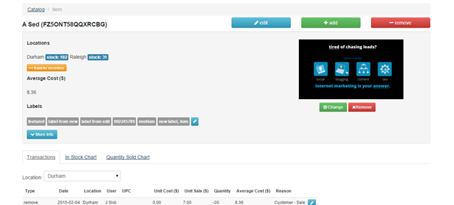
\includegraphics[width=0.49\linewidth]{slike/ST_slika.png}
			\centering
			\label{st_logo}
		\end{figure}
		
		\bigskip
				
		\large\textbf{\textit{Tržište i ciljana skupina}}\normalsize
		
		Ciljana skupina su tvrtke koje posjeduju veliki broj skladišta na brojnim i udaljenim lokacijama te im je tako proces inventure otežan. Tržište su sve kompanije koje posjeduju skladišta, posebice kompanije koje rade kontinuirane inventure.\\
		
		\large\textbf{\textit{Opseg projektnog zadatka}}\normalsize
		
		Aplikacija se sastoji od intuitivnog korisničkog sučelja, a osnovne su funkcionalnosti detekcija i skeniranje QR ili bar kodova artikala u skladištu prilikom inventure. Svaki korisnik mora moći skenirati artikle, a ostale funkcionalnosti se dijele prema razini pristupa. Direktor ima pristup svim funkcionalnostima aplikacije, između ostaloga uvid u sva skladišta, artikle i statistiku pogrešaka pojedinog skladištara. Važna funkcionalnost je dodavanje artikala u stablo proizvoda. Pristup toj funkcionalnosti ima samo direktor tvrtke. Također, aplikacija mora omogućiti svakom skladištaru skeniranje samo jedne vrste artikala dok ne završi s prebrojavanjem te vrste artikla. Svaki korisnik može se prijaviti, registrirati ako nema napravljen račun, kao i odjaviti ako želi.\\
		
		\large\textbf{\textit{Moguće nadogradnje projektnog zadatka}}\normalsize
		
		Projektni zadatak mogao bi se nadograditi integracijom s nekom od popularnih aplikacija za upravljanje timom (npr. \emph{Slack}). Tako bismo ubacili opciju međusobne komunikacije između članova tvrtke. Osim automatski generiranih poruka koje aplikacija nudi, svi članovi kompanije mogli bi razmjenjivati poruke međusobno. Uz to, jedna od mogućih nadogradnji svakako je višejezičnost. Aplikacija bi mogla evidentirati nabavne i prodajne naloge te automatski dodavati odnosno oduzimati broj artikala ovisno o njihovoj prodaji ili nabavi.\\
		
		
		Za pomoć pogledati reference navedene u poglavlju „Popis literature“, a po potrebi konzultirati sadržaj na internetu koji nudi dobre smjernice u tom pogledu.
		\eject
		
		\begin{comment}
		\section{Primjeri u \LaTeX u}
		
		\textit{Ovo potpoglavlje izbrisati.}\\

		U nastavku se nalaze različiti primjeri kako koristiti osnovne funkcionalnosti \LaTeX a koje su potrebne za izradu dokumentacije. Za dodatnu pomoć obratiti se asistentu na projektu ili potražiti upute na sljedećim web sjedištima:
		\begin{itemize}
			\item Upute za izradu diplomskog rada u \LaTeX u - \url{https://www.fer.unizg.hr/_download/repository/LaTeX-upute.pdf}
			\item \LaTeX\ projekt - \url{https://www.latex-project.org/help/}
			\item StackExchange za Tex - \url{https://tex.stackexchange.com/}\\
		
		\end{itemize} 	


		
		\noindent \underbar{podcrtani tekst}, \textbf{podebljani tekst}, 	\textit{nagnuti tekst}\\
		\noindent \normalsize primjer \large primjer \Large primjer \LARGE {primjer} \huge {primjer} \Huge primjer \normalsize
				
		\begin{packed_item}
			
			\item  primjer
			\item  primjer
			\item  primjer
			\item[] \begin{packed_enum}
				\item primjer
				\item[] \begin{packed_enum}
					\item[1.a] primjer
					\item[b] primjer
				\end{packed_enum}
				\item primjer
			\end{packed_enum}
			
		\end{packed_item}
		
		\noindent primjer url-a: \url{https://www.fer.unizg.hr/predmet/proinz/projekt}
		
		\noindent posebni znakovi: \# \$ \% \& \{ \} \_ 
		$|$ $<$ $>$ 
		\^{} 
		\~{} 
		$\backslash$ 
		
		
		\begin{longtblr}[
			label=none,
			entry=none
			]{
				width = \textwidth,
				colspec={|X[8,l]|X[8, l]|X[16, l]|}, 
				rowhead = 1,
			} %definicija širine tablice, širine stupaca, poravnanje i broja redaka naslova tablice
			\hline \multicolumn{3}{|c|}{\textbf{naslov unutar tablice}}	 \\ \hline[3pt]
			\SetCell{LightGreen}IDKorisnik & INT	&  	Lorem ipsum dolor sit amet, consectetur adipiscing elit, sed do eiusmod  	\\ \hline
			korisnickoIme	& VARCHAR &   	\\ \hline 
			email & VARCHAR &   \\ \hline 
			ime & VARCHAR	&  		\\ \hline 
			\SetCell{LightBlue} primjer	& VARCHAR &   	\\ \hline 
		\end{longtblr}
		

		\begin{longtblr}[
				caption = {Naslov s referencom izvan tablice},
				entry = {Short Caption},
			]{
				width = \textwidth, 
				colspec = {|X[8,l]|X[8,l]|X[16,l]|}, 
				rowhead = 1,
			}
			\hline
			\SetCell{LightGreen}IDKorisnik & INT	&  	Lorem ipsum dolor sit amet, consectetur adipiscing elit, sed do eiusmod  	\\ \hline
			korisnickoIme	& VARCHAR &   	\\ \hline 
			email & VARCHAR &   \\ \hline 
			ime & VARCHAR	&  		\\ \hline 
			\SetCell{LightBlue} primjer	& VARCHAR &   	\\ \hline 
		\end{longtblr}
	


		
		
		%unos slike
		\begin{figure}[H]
			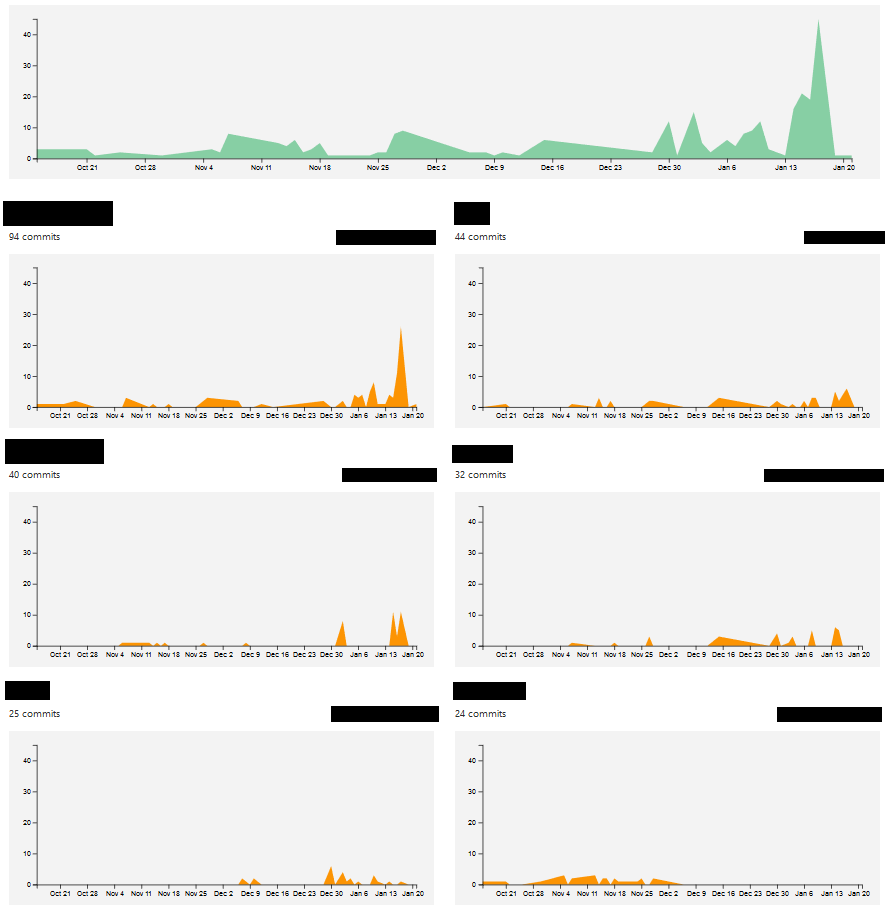
\includegraphics[scale=0.4]{slike/aktivnost.png} %veličina slike u odnosu na originalnu datoteku i pozicija slike
			\centering
			\caption{Primjer slike s potpisom}
			\label{fig:promjene}
		\end{figure}
		
		\begin{figure}[H]
			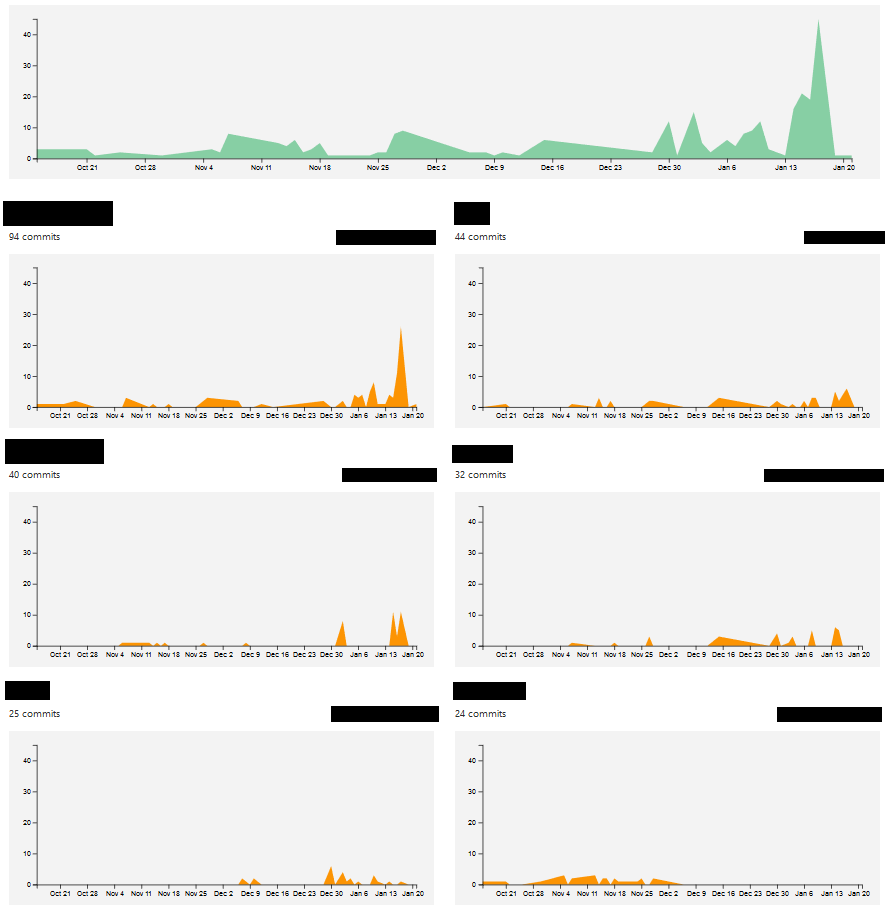
\includegraphics[width=\textwidth]{slike/aktivnost.png} %veličina u odnosu na širinu linije
			\caption{Primjer slike s potpisom 2}
			\label{fig:promjene2} %label mora biti drugaciji za svaku sliku
		\end{figure}
		
		Referenciranje slike \ref{fig:promjene2} u tekstu.
		
		\eject
		\end{comment}
		
	
	\chapter{Specifikacija programske potpore}
		
	\section{Funkcionalni zahtjevi}
			
			
			\noindent \textbf{Dionici:}
			
			\begin{packed_enum}
				
				\item Skladištar
				\item Šef skladišta			
				\item Direktor
				\item Razvojni tim
				
			\end{packed_enum}
			
			\noindent \textbf{Aktori i njihovi funkcionalni zahtjevi:}
			
			
			\begin{packed_enum}
				\item	\underbar{Skladištar (inicijator) može:}
					
					\begin{packed_enum}
						\item Skenirati artikle za inventuru
						\item Pristupiti povijesti svih svojih unosa
						\item Dojaviti šefu skladišta da artikla nema na skladištu
						\item Odjaviti se
					\end{packed_enum}

				\item  \underbar{Šef skladišta (inicijator) može:}
					
					\begin{packed_enum}
						\item Skenirati artikle za inventuru
							\begin{packed_enum}
								\item Kao kontrolor
								\item Kao izvršitelj inventure
							\end{packed_enum}
						\item Vidjeti sve artikle na skladištu u kojem je nadležan
						\item Pristupiti povijesti svih svojih unosa
						\item Primati obavijesti o nedostatku pojedinog artikla koje dojavi skladištar
							\begin{packed_enum}
								\item Proslijediti tu obavijest direktoru
							\end{packed_enum}
						\item Odjaviti se
					\end{packed_enum}

				\item  \underbar{Direktor (inicijator) može:}
				
				\begin{packed_enum}
					\item Skenirati artikle za inventuru
					\item Vidjeti povijest svih svojih unosa
					\item Vidjeti stanje artikala na svim skladištima
					\item Vidjeti statistiku pogrešaka svakog skladištara
					\item Izabrati skladišta koje želi provjeriti
						\begin{packed_enum}
							\item Izabrati inventure na odabranom skladištu
							\item Pregledati sve skenirane artikle u toj inventuri
						\end{packed_enum}
					\item Dodati novo skladište
					\item Urediti stablo artikala
						\begin{packed_enum}
							\item Dodati artikl
							\item Ukloniti Artikl
							\item Dodati kategoriju
							\item Ukloniti kategoriju
						\end{packed_enum}
					\item Pristupiti svim obavijestima
					\begin{packed_enum}
						\item Razriješiti obavijesti
					\end{packed_enum}
					\item Odjaviti se
				\end{packed_enum}
			
			
			\item	\underbar{Baza podataka (sudionik)}
				\begin{packed_enum}
					\item Pohranjivati sve podatke o korisnicima i njihovim ovlastima
					\item Pohranjivati sve podatke o inventurama, skladištima, obavijestima i artiklima
				\end{packed_enum}
			\end{packed_enum}
			
			\eject 
			
			
				
			\subsection{Obrasci uporabe}
				
				
				\subsubsection{Opis obrazaca uporabe}
					
					\noindent \underbar{\textbf{UC1 - Registracija}}
					\begin{packed_item}
	
						\item \textbf{Glavni sudionik: }Korisnik
						\item  \textbf{Cilj:} Stvoriti korisnički račun za pristup sustavu
						\item  \textbf{Sudionici:} Baza podataka
						\item  \textbf{Preduvjet:} -
						\item  \textbf{Opis osnovnog tijeka:}
						
						\item[] \begin{packed_enum}
	
							\item Korisnik odabire opciju za registraciju
							\item Korisnik unosi potrebne korisničke podatke te bira jednu od ponuđenih uloga
							\item Podaci se spremaju u bazu podataka
														
						\end{packed_enum}
						
						\item  \textbf{Opis mogućih odstupanja:}
						
						\item[] \begin{packed_item}
	
							\item[2.a] Odabir email adrese koja se već koristi, unos podataka u nedozvoljenom formatu, ne popunjavanje svih potrebnih podataka 
							\item[] \begin{packed_enum}
								
								\item Sustav obavještava korisnika o neuspjelom upisu i vraća ga na stranicu za prijavu
								\item Korisnik mijenja potrebne podatke te završava unos ili odustaje od registracije
								
							\end{packed_enum}
						\end{packed_item}
					\end{packed_item}
				

					\noindent \underbar{\textbf{UC2 - Prijava u sustav}}
					\begin{packed_item}
	
						\item \textbf{Glavni sudionik: }Skladištar, šef skladišta, direktor
						\item  \textbf{Cilj:} Prijaviti se u sustav i dobiti pristup korisničkom sučelju
						\item  \textbf{Sudionici:} Baza podataka
						\item  \textbf{Preduvjet:} Registracija
						\item  \textbf{Opis osnovnog tijeka:}
						
						\item[] \begin{packed_enum}
	
							\item Korisnik unosi email adresu i lozinku
							\item Uspoređuje se korisnikov unos s podacima u bazi podataka 
							\item Prikazuje se početni zaslon aplikacije
							
						\end{packed_enum}
						
						\item  \textbf{Opis mogućih odstupanja:}
						
						\item[] \begin{packed_item}
	
							\item[2.a] Neispravna email adresa  ili lozinka
							\item[] \begin{packed_enum}
								
								\item Sustav obavještava korisnika o neuspjelom upisu i vraća ga na stranicu za registraciju\\
								
							\end{packed_enum}
						\end{packed_item}
					\end{packed_item}
				
		
					\noindent \underbar{\textbf{UC3 - Odjava iz sustava}}
					\begin{packed_item}
	
						\item \textbf{Glavni sudionik: }Skladištar, šef skladišta, direktor
						\item  \textbf{Cilj:} Odjaviti se iz sustava
						\item  \textbf{Sudionici:} Baza podataka
						\item  \textbf{Preduvjet:} Korisnik je prijavljen u sustav
						\item  \textbf{Opis osnovnog tijeka:}
						
						\item[] \begin{packed_enum}
	
							\item Korisnik odabire opciju "Odjava" s ikonom mobilnog uređaja i strelice u gornjem desnom kutu
							\item Prikazuje se stranica za registraciju 
														
						\end{packed_enum}
					\end{packed_item}	
					
					\noindent \underbar{\textbf{UC4 - Skeniranje artikla}}
					\begin{packed_item}
	
						\item \textbf{Glavni sudionik: }Skladištar, šef skladišta, direktor
						\item  \textbf{Cilj:} Skenirati artikl
						\item  \textbf{Sudionici:} Baza podataka
						\item  \textbf{Preduvjet:} Korisnik je prijavljen u sustav i odabrao je koji artikl želi skenirati
						\item  \textbf{Opis osnovnog tijeka:}
						
						\item[] \begin{packed_enum}
							
							\item Korisnik postavlja mobilni uređaj iznad bar ili QR koda koji želi skenirati
							\item Korisnik pritiskom na ikonu QR koda (sredina, dolje) skenira kod artikla
							\item Prikazuje se pop-up window s informacijama o skeniranom artiklu
							\item Korisnik u pop-up window-u odabire mogućnost povećanja ili smanjenja broja takvih artikala na skladištu pritiskom na ikone "-" i "+", odbacivanja trenutno skeniranog proizvoda bez spremanja u bazu pritiskom na opciju "Odbaci", spremanje artikla u bazu pritiskom na opciju "Spremi" te izlaska iz pop-up window-a pritiskom na opciju "Završi"
							
						\end{packed_enum}
						
						\item  \textbf{Opis mogućih odstupanja:}
						
						\item[] \begin{packed_item}
	
							\item[2.a] Skenirani artikl ne postoji u bazi podataka
							\item[] \begin{packed_enum}
								
								\item Sustav obavještava korisnika o neuspjelom pokušaju skeniranja uz poruku "Skenirani artikl ne postoji u bazi podataka" te ga vraća na početni zaslon za skeniranje artikala								
							\end{packed_enum}
						
							\item[2.b] Skenirani artikl nije onaj odabrani
							\item[] \begin{packed_enum}
								\item Sustav obavještava korisnika o neuspjelom pokušaju skeniranja uz poruku "Skenirani artikl nije onaj odabrani" te ga vraća na početni zaslon za skeniranje artikala\\  
							\end{packed_enum}
						\end{packed_item}
					\end{packed_item}
				
					\noindent \underbar{\textbf{UC5 - Završetak skeniranja artikla}}
					\begin{packed_item}
						\item \textbf{Glavni sudionik: }Skladištar, šef skladišta, direktor
						\item  \textbf{Cilj:} Završiti sa skeniranjem odabranog artikla
						\item  \textbf{Sudionici:} Baza podataka
						\item  \textbf{Preduvjet:} Korisnik je prijavljen u sustav i odabrao je artikl koji želi skenirati
						\item  \textbf{Opis osnovnog tijeka:}
						\item[] \begin{packed_enum}
							\item Korisnik na početnom zaslonu pritišće gumb "Završi"
							\item Korisnik potvrđuje da želi završiti sa skeniranjem odabranog artikla
						\end{packed_enum}
					\end{packed_item}
					
					
					\noindent \underbar{\textbf{UC6 - Pregled povijesti inventura}}
					\begin{packed_item}
	
						\item \textbf{Glavni sudionik: }Skladištar, šef skladišta
						\item  \textbf{Cilj:} Pregled svih unosa artikala po inventurama
						\item  \textbf{Sudionici:} Baza podataka
						\item  \textbf{Preduvjet:} Korisnik je prijavljen u sustav
						\item  \textbf{Opis osnovnog tijeka:}
						
						\item[] \begin{packed_enum}
	
							\item Korisnik pritišće ikonu liste u donjem lijevom kutu početnog zaslona
							\item Prikazuje se popis inventura 
							\item Korisnik bira inventuru
							\item Prikazuje se popis skeniranih artikala 
														
						\end{packed_enum}
					\end{packed_item}
					
					
					\noindent \underbar{\textbf{UC7 - Pregled povijesti inventura}}
					\begin{packed_item}
	
						\item \textbf{Glavni sudionik: }Direktor
						\item  \textbf{Cilj:} Pregled svih unosa artikala po inventurama u svim skladištima 
						\item  \textbf{Sudionici:} Baza podataka
						\item  \textbf{Preduvjet:} Korisnik je prijavljen u sustav
						\item  \textbf{Opis osnovnog tijeka:}
						
						\item[] \begin{packed_enum}
	
							\item Korisnik pritišće ikonu liste u donjem lijevom kutu početnog zaslona
							\item Prikazuje se popis svih skladišta
							\item Korisnik bira skladište
							\item Prikazuje se popis inventura 
							\item Korisnik bira inventuru
							\item Prikazuje se popis skeniranih artikala \\
							\newline
							\newline
																				
						\end{packed_enum}
					\end{packed_item}
					
					
					\noindent \underbar{\textbf{UC8 - Dojava da određenog artikla nema na skladištu}}
					\begin{packed_item}
	
						\item \textbf{Glavni sudionik: }Skladištar, šef skladišta
						\item  \textbf{Cilj:} Dojaviti nadređenima da određenog artikla nema na skladištu
						\item  \textbf{Sudionici:} Baza podataka
						\item  \textbf{Preduvjet:} Korisnik je prijavljen u sustav
						\item  \textbf{Opis osnovnog tijeka:}
						
						\item[] \begin{packed_enum}
	
							\item Korisnik odabire opciju "Nema artikla"
							\item Korisnik odabire naziv artikla
							\item Korisnik odabire opciju "Dojavi"
														
						\end{packed_enum}
					\end{packed_item}
					
					
					\noindent \underbar{\textbf{UC9 - Pregled obavijesti}}
					\begin{packed_item}
	
						\item \textbf{Glavni sudionik: }Šef skladišta
						\item  \textbf{Cilj:} Pregled obavijesti koje su poslali skladištari
						\item  \textbf{Sudionici:} Baza podataka
						\item  \textbf{Preduvjet:} Korisnik je prijavljen u sustav
						\item  \textbf{Opis osnovnog tijeka:}
						
						\item[] \begin{packed_enum}
	
							\item Korisnik odabire opciju s ikonom pošte 
							\item Prikazuje se stranica s obavijestima o artiklima kojih nema na skladištu
							\item Korisnik odabire opciju "Šalji direktoru" ako to smatra opravdanim
							\item Odabrana obavijest se šalje direktoru
														
						\end{packed_enum}
					\end{packed_item}
					
					
					\noindent \underbar{\textbf{UC10 - Pregled obavijesti}}
					\begin{packed_item}
	
						\item \textbf{Glavni sudionik: }Direktor
						\item  \textbf{Cilj:} Pregled obavijesti koje su poslali šefovi skladišta
						\item  \textbf{Sudionici:} Baza podataka
						\item  \textbf{Preduvjet:} Korisnik je prijavljen u sustav
						\item  \textbf{Opis osnovnog tijeka:}
						
						\item[] \begin{packed_enum}
	
							\item Korisnik odabire opciju s ikonom pošte 
							\item Prikazuje se stranica s obavijestima o artiklima kojih nema na skladištu i o pogreškama skladištara 
							\item Korisnik odabire kvačicu ako želi određenu obavijest označiti kao riješenu, križić ako ju želi označiti kao odbačenu, ili opcije "Razriješi sve" i "Odbaci sve"\\
							\newline
														
						\end{packed_enum}
					\end{packed_item}
					
					
					\noindent \underbar{\textbf{UC11 - Pregled svih artikala na skladištu}}
					\begin{packed_item}
	
						\item \textbf{Glavni sudionik: }Šef skladišta
						\item  \textbf{Cilj:} Pregled broj svih artikala na skladištu
						\item  \textbf{Sudionici:} Baza podataka
						\item  \textbf{Preduvjet:} Korisnik je prijavljen u sustav
						\item  \textbf{Opis osnovnog tijeka:}
						
						\item[] \begin{packed_enum}
	
							\item Korisnik odabire opciju s ikonom kuće
							\item Prikazuje se popis artikala u skladištu temeljem zadnje odrađene inventure i njihova količina 
																					
						\end{packed_enum}
					\end{packed_item}
					
					
					\noindent \underbar{\textbf{UC12 - Pregled svih skladišta kompanije}}
					\begin{packed_item}
	
						\item \textbf{Glavni sudionik: }Direktor
						\item  \textbf{Cilj:} Pregled svih skladišta kompanije te artikala i skladištara u njima 
						\item  \textbf{Sudionici:} Baza podataka
						\item  \textbf{Preduvjet:} Korisnik je prijavljen u sustav
						\item  \textbf{Opis osnovnog tijeka:}
						
						\item[] \begin{packed_enum}
							
							\item Korisnik odabire opciju s ikonom kuće
							\item Prikazuje se popis skladišta
							\item Korisnik bira skladište
							\item Prikazuje se popis artikala i skladištara u odabranom skladištu 
							\item Korisnik odabire opciju "Artikl"
							\item Prikazuje se popis artikala u odabranom skladištu 
							\item Korisnik odabire opciju "Skladištar"
							\item Prikazuje se popis skladištara i njihova statistika pogreške u odabranom skladištu 
																												
						\end{packed_enum}
					\end{packed_item}
					
					
					\noindent \underbar{\textbf{UC13 - Dodavanje skladišta}}
					\begin{packed_item}
	
						\item \textbf{Glavni sudionik: }Direktor
						\item  \textbf{Cilj:} Dodati novo skladišta
						\item  \textbf{Sudionici:} Baza podataka
						\item  \textbf{Preduvjet:} Korisnik je prijavljen u sustav
						\item  \textbf{Opis osnovnog tijeka:}
						
						\item[] \begin{packed_enum}
	
							\item Korisnik odabire opciju "+" na stranici s popisom skladišta
							\item Prikazuje se stranica za unos novog skladišta
							\item Korisnik unosi novo skladište
							\item Korisnik izabire drugog korisnika s oznakom "Šef skladišta" za odabranu lokaciju
							\item Novo skladište se sprema u bazu podataka
																												
						\end{packed_enum}
					\end{packed_item}
				
					\noindent \underbar{\textbf{UC14 - Brisanje skladišta}}
					\begin{packed_item}
						
						\item \textbf{Glavni sudionik: }Direktor
						\item  \textbf{Cilj:} Obrisati skladište
						\item  \textbf{Sudionici:} Baza podataka
						\item  \textbf{Preduvjet:} Korisnik je prijavljen u sustav i skladište postoji
						\item  \textbf{Opis osnovnog tijeka:}
						
						\item[] \begin{packed_enum}
							\item Korisnik odabire skladište koje želi obrisati
							\item Korisnik pritiskom na ikonu kante za smeće briše odabrano skladište
						\end{packed_enum}
						
						
					\end{packed_item}
					
					
					\noindent \underbar{\textbf{UC15 - Dodavanje artikla}}
					\begin{packed_item}
	
						\item \textbf{Glavni sudionik: }Direktor
						\item  \textbf{Cilj:} Dodati novi artikl ili kategoriju proizvoda 
						\item  \textbf{Sudionici:} Baza podataka
						\item  \textbf{Preduvjet:} Korisnik je prijavljen u sustav
						\item  \textbf{Opis osnovnog tijeka:}
						
						\item[] \begin{packed_enum}
	
							\item Korisnik odabire opciju "+" na stranici s popisom artikala
							\item Prikazuje se stranica za unos novog artikla 
							\item Korisnik unosi novi artikl ili kategoriju
							\item Promjene se spremaju u bazu podataka
																					
						\end{packed_enum}
					\end{packed_item}
					
					\noindent \underbar{\textbf{UC16 - Preraspodjela artikla}}
					\begin{packed_item}
						\item \textbf{Glavni sudionik: }Direktor
						\item  \textbf{Cilj:} Preraspodijeliti postojeći artikl 
						\item  \textbf{Sudionici:} Baza podataka
						\item  \textbf{Preduvjet:} Korisnik je prijavljen u sustav i artikl postoji u sustavu
						\item  \textbf{Opis osnovnog tijeka:}
						
						\item[] \begin{packed_enum}
							\item Korisnik odabire koji proizvod želi preraspodijeliti
							\item Otvara se pop-up window sa mogućnosti odabira nove kategorije
							\item Korisnik odabire u novu kategoriju
							\item Korisnik potvrđuje novu kategoriju
							\item Proizvod ili kategorija proizvoda se preraspodijeli u novu kategoriju
							\newline
						\end{packed_enum}
					
						
					\end{packed_item}
				
					\noindent \underbar{\textbf{UC17 - Brisanje artikla}}
					\begin{packed_item}
						\item \textbf{Glavni sudionik: }Direktor
						\item  \textbf{Cilj:} Obrisati postojeći artikl ili kategoriju proizvoda 
						\item  \textbf{Sudionici:} Baza podataka
						\item  \textbf{Preduvjet:} Korisnik je prijavljen u sustav i artikl postoji u sustavu
						\item  \textbf{Opis osnovnog tijeka:}
						
						\item[] \begin{packed_enum}
							\item Korisnik odabire koji proizvod ili kategoriju proizvoda želi obrisati
							\item Otvara se pop-up window sa upozorenjem
							\item Korisnik potvrđuje da želi obrisati proizvod
						\end{packed_enum}
					\item  \textbf{Opis mogućih odstupanja:} 
					\item[] \begin{packed_item}
						
						\item[2.a] Čvor kategorije proizvoda koji se želi obrisati ima djecu
						\item[] \begin{packed_enum}
							
							\item Sustav obavještava korisnika o pogrešci i ne dozvoljava brisanje kategorije proizvoda
							
						\end{packed_enum}
					\end{packed_item}
					
					\end{packed_item}
				
					\noindent \underbar{\textbf{UC18 - Završetak inventure}}
					\begin{packed_item}
						\item \textbf{Glavni sudionik: }Direktor
						\item  \textbf{Cilj:} Završiti inventuru i započeti sljedeću
						\item  \textbf{Sudionici:} Baza podataka
						\item  \textbf{Preduvjet:} Korisnik je prijavljen u sustav i inventura traje
						\item  \textbf{Opis osnovnog tijeka:}
						
						\item[] \begin{packed_enum}
							\item Korisnik na početnom zaslonu odabire gumb "završi inventuru"
							\item Korisnik potvrđuje da želi završiti inventuru
							\item Trenutna inventura završava te se svi njezini unosi šalju u bazu podataka
							\item Automatski počinje nova inventura
						\end{packed_enum}
					\end{packed_item}

				\subsubsection{Dijagrami obrazaca uporabe}
					
					\begin{figure}[H]
						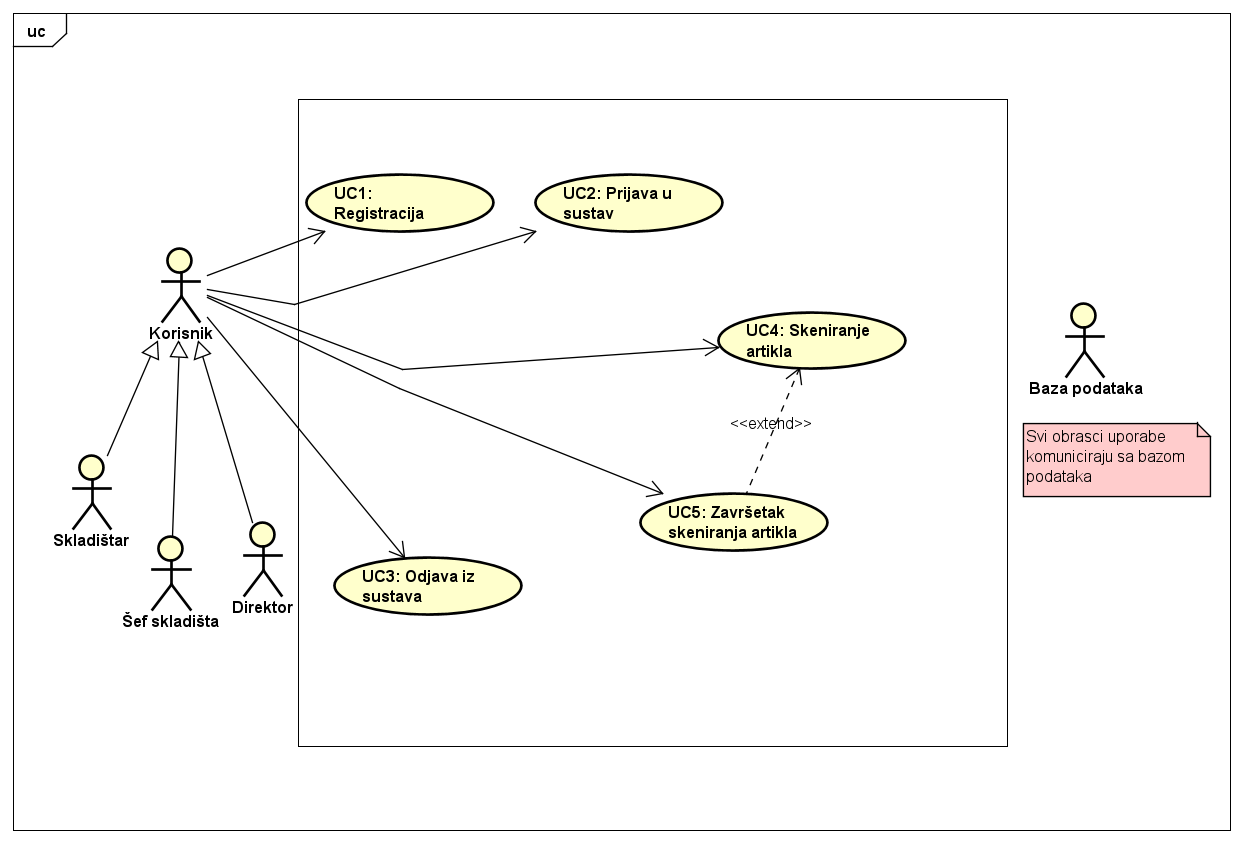
\includegraphics[scale=0.5]{slike/uc1.png}
						\caption{Dijagram obrasca uporabe, zajedničke funkcionalnost svih korisnika}
						
					\end{figure}
				
					\begin{figure}[H]
						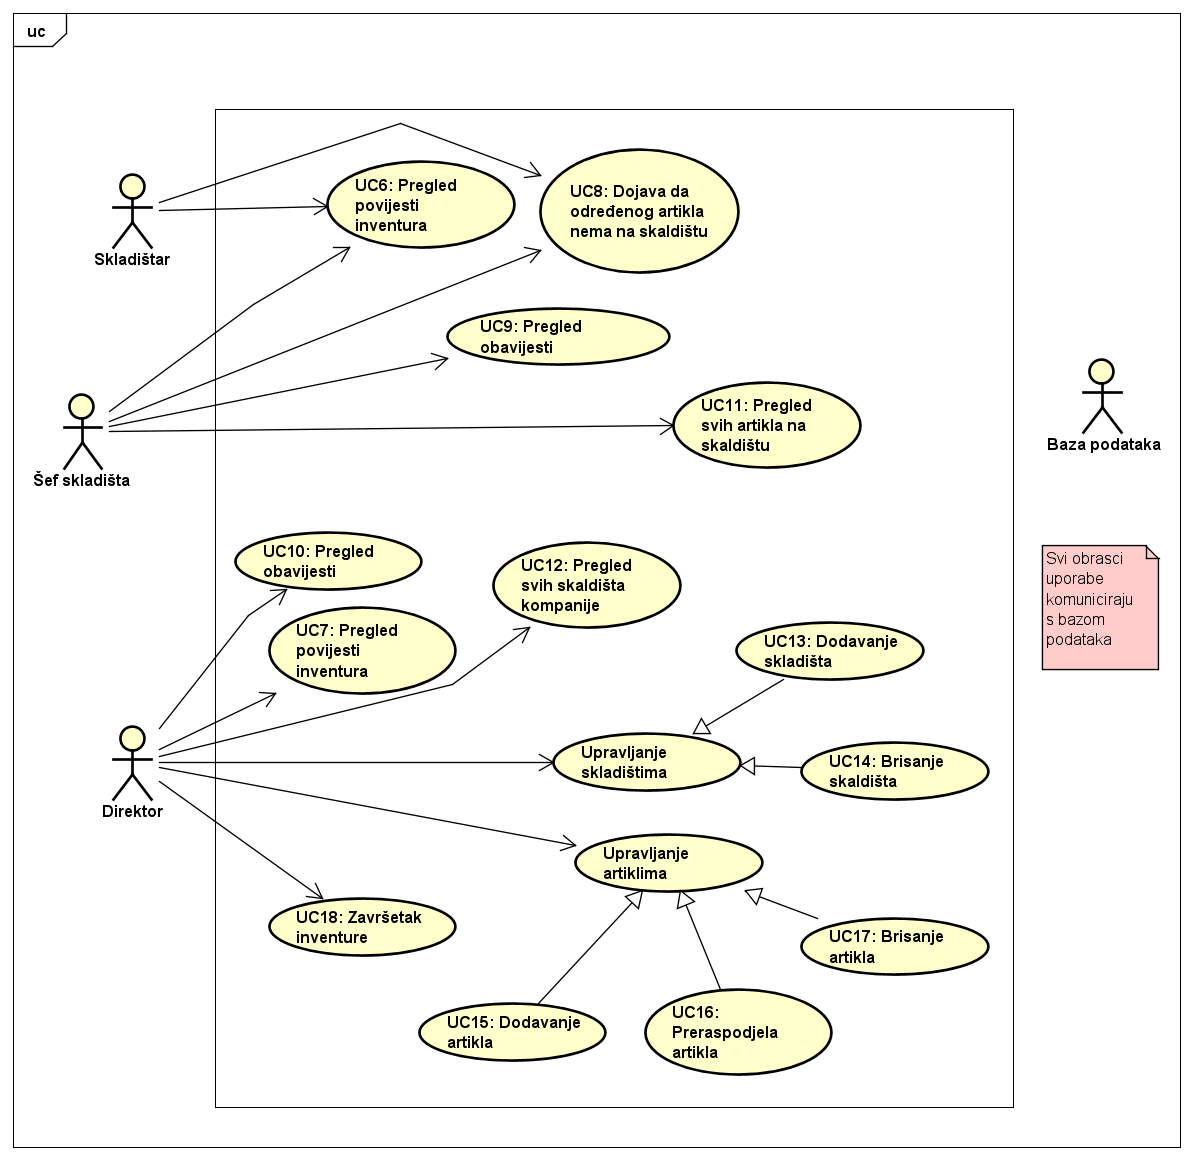
\includegraphics[scale=0.5]{slike/uc2.png}
						\caption{Dijagram obrasca uporabe, zasebne funkcionalnost skladištara, šefa skladišta i direktora}
					\end{figure}
				
			\subsection{Sekvencijski dijagrami}
				
				\textbf{Obrazac uporabe UC4 - Skeniranje artikla}
				
				Korisnik detekcijom koda šalje zahtjev mobilnoj aplikaciji za prikaz informacija o artiklu kako bi mogao uređivati broj tog artikla na skladištu. Ukoliko u bazi podataka ne postoji artikl sa odgovarajućim kodom mobilna aplikacija korisniku na zaslon ispiše odgovarajuću obavijest. Inače ako skenirani artikl nije onaj koji se trenutno skenira mobilna aplikacija također korisniku ispiše odgovarajuću obavijest. Ako u bazi podataka postoji artikl sa odgovarajućim kodom i ako je taj artikl onaj koji se trenutno skenira, mobilna aplikacija dohvaća podatake o artiklu i u obliku pop-up prozora prikazuje te informacije. Na zaslonu s informacijama o skeniranom proizvodu korisniku se nudi opcija da poveća ili smanji broj takvih artikala u skladištu, da odbaci trenutno očitanje bez spremanja u bazu ili da trenutno očitanje odmah pohrani u bazu (bez čekanja da istekne 5 sekundi). Promjenom broja očitanih artikala resetira se brojač 5 sekundi. Istekom vremena brojača zapis se automatski pohranjuje u bazu.
				
			\begin{figure}[H]
				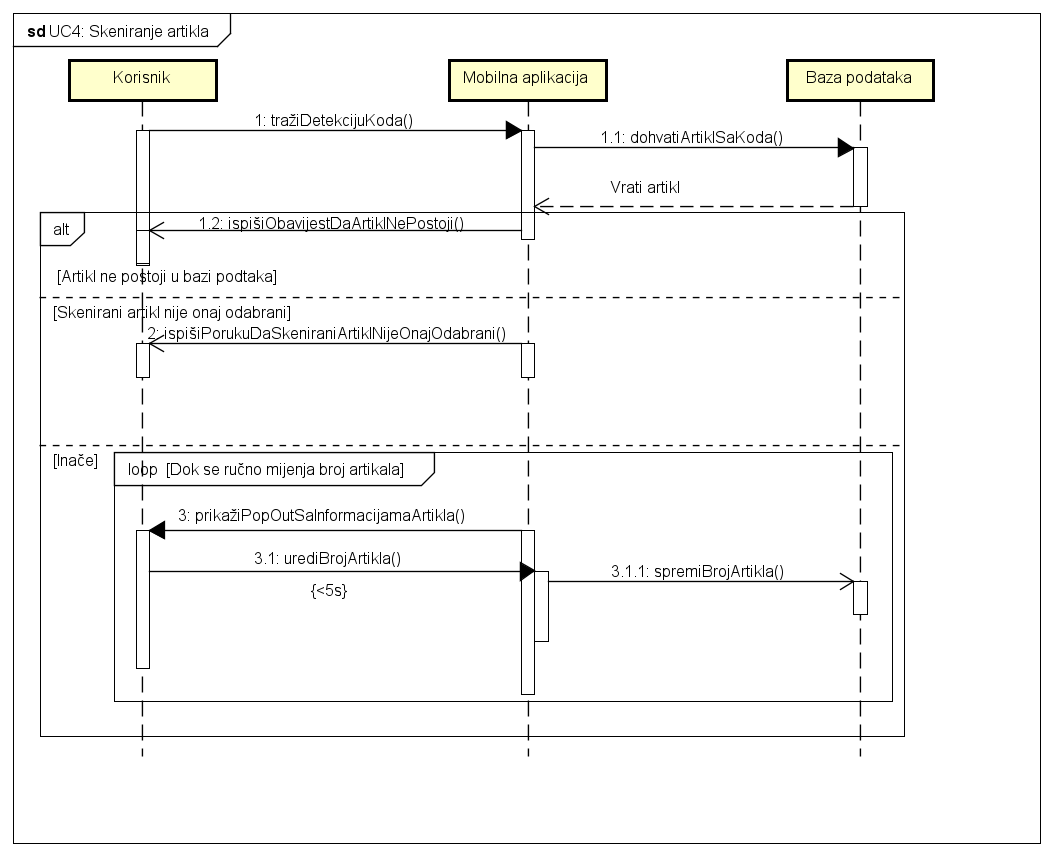
\includegraphics[scale=0.5]{slike/sekUC4.png}
				\caption{Sekvencijski dijagram za UC4}
			\end{figure}
				
			\textbf{Obrazac uporabe UC16 - Preraspodjela artikla}
			
			Korisnik šalje zahtjev mobilnoj aplikaciji za prikazom stabla proizvoda. Mobilna aplikacija dohvaća stablo proizvoda i prikazuje ga korisniku. Korisnik dok ne dođe do željenog proizvoda šalje zahtjeve za prikaz djece odabranog čvora. Kada korisnik odabere željeni list stabla mobilna aplikacija iz baze podataka dohvaća sve čvorove razine iznad izabranog lista. Mobilna aplikacija prikazuje sve čvorove razine iznad izabranog lista. Korisnik odabire novog roditelja. Nova struktura stabla se pohranjuje u bazu podataka.
			
			\begin{figure}[H]
				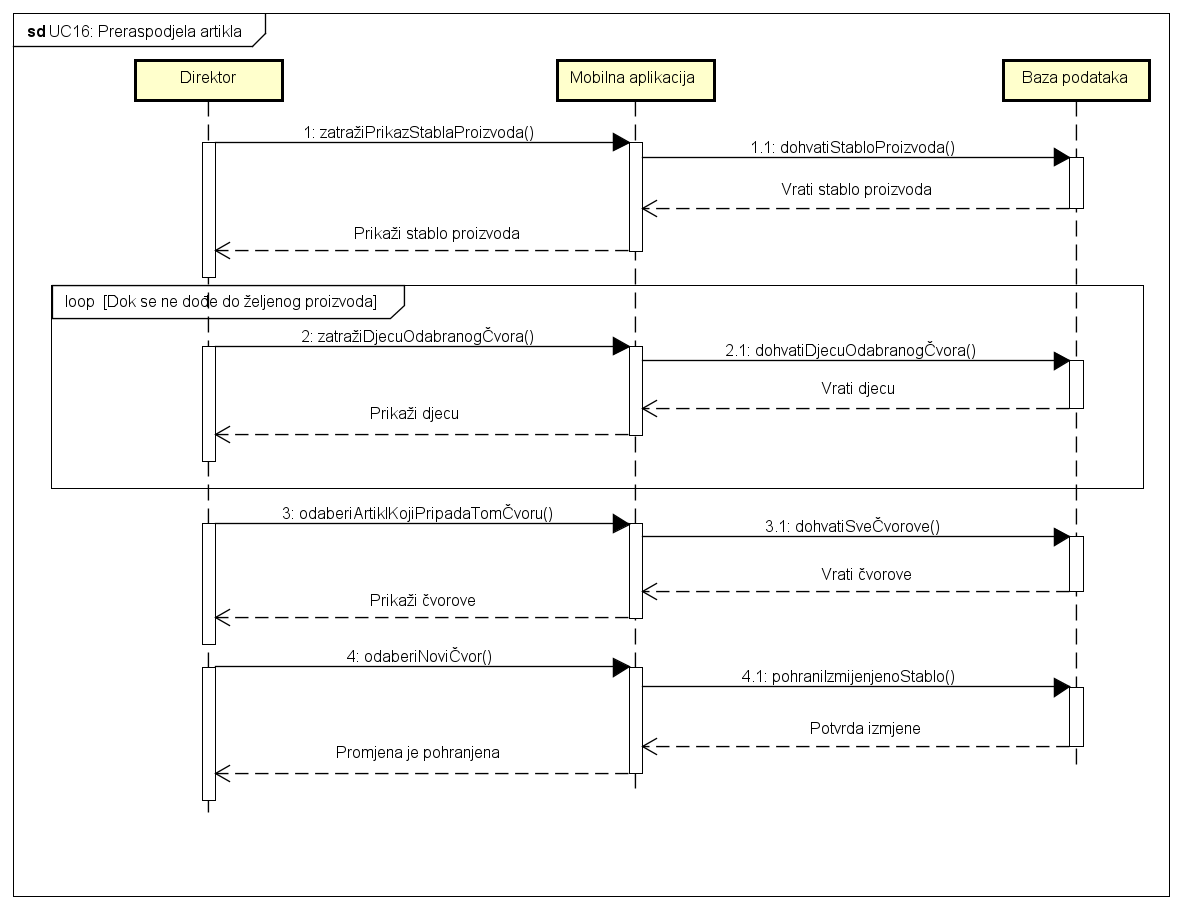
\includegraphics[scale=0.5]{slike/sekUC16.png}
				\caption{Sekvencijski dijagram za UC16}
			\end{figure}
		
			\textbf{Sekvencijski dijagram - završetak trenutne inventure}
			
			Korisnik od aplikacije traži završetak inventure. Aplikacija se povezuje s bazom podataka te od nje traži završetak trenutne inventure. U slučaju pogreške, to se dojavljuje korisniku pomoću pop-up prikaza. Ako je trenutna inventura uspješno završena, baza podataka to dojavljuje aplikacija, a ona dalje korisniku. Aplikacija nakon toga implicitno pokreće novu inventuru. Ukoliko se prilikom stvaranja nove inventure dogodi pogreška, status pogreške se dojavljuje korisniku.
			
			\begin{figure}[H]
				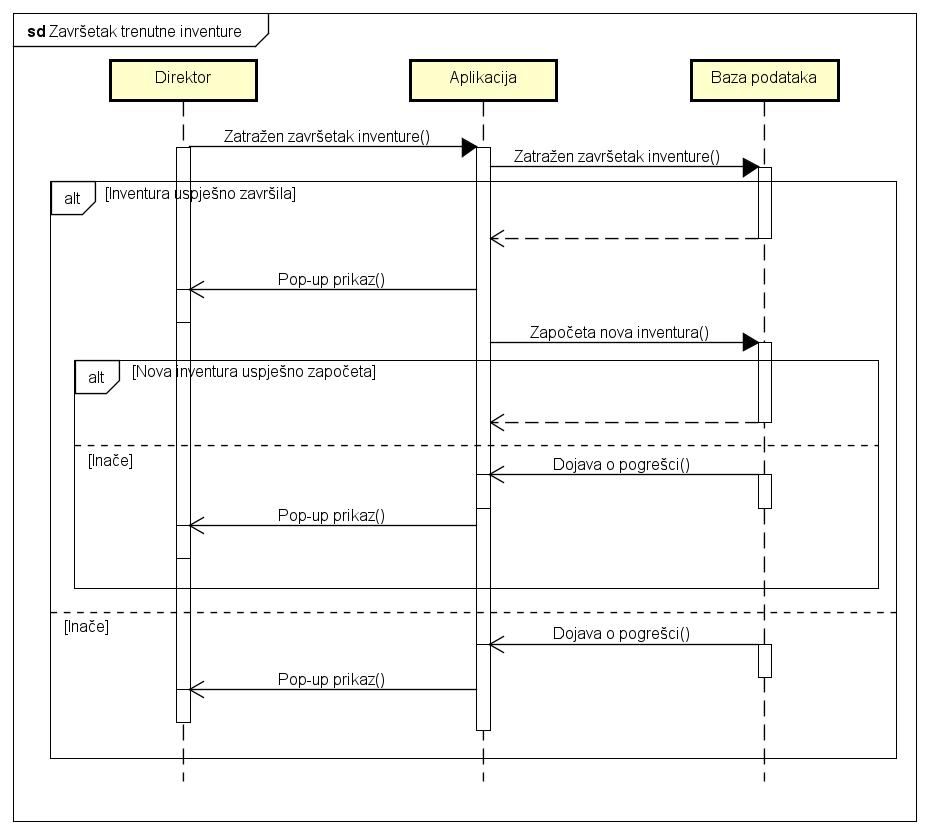
\includegraphics[scale=0.5]{slike/Sekvencijski dijagram.jpg}
				\caption{Sekvencijski dijagram za završetak trenutne inventure}
			\end{figure}
	
		\section{Ostali zahtjevi}
		
			\begin{packed_item}
				\item Sustav treba omogućiti rad više korisnika u stvarnom vremenu
				\item Korisničko sučelje i sustav moraju podržavati hrvatsku abecedu (dijakritičke znakove) pri unosu i prikazu tekstualnog sadržaja
				\item Sustav treba dohvaćati lokaciju korisnika preko GPS modula
				\item Izvršavanje dijela programa u kojem se pristupa bazi podataka ne smije trajati duže od nekoliko sekundi 
				\item Sustav treba biti implementiran kao mobilna aplikacija koristeći objektno-orijentirane jezike

				\item Neispravno korištenje korisničkog sučelja ne smije narušiti funkcionalnost i rad sustava

				\item Sustav treba biti jednostavan za korištenje, korisnici se moraju znati koristiti sučeljem bez opširnih uputa 
				\item Veza s bazom podataka mora biti kvalitetno zaštićena, brza i otporna na vanjske greške
			\end{packed_item}
			 
			 
			 
	
	\chapter{Arhitektura i dizajn sustava}
		\begin{comment}
		\textbf{\textit{dio 1. revizije}}\\

		\textit{ Potrebno je opisati stil arhitekture te identificirati: podsustave, preslikavanje na radnu platformu, spremišta podataka, mrežne protokole, globalni upravljački tok i sklopovsko-programske zahtjeve. Po točkama razraditi i popratiti odgovarajućim skicama:}
	\begin{itemize}
		\item 	\textit{izbor arhitekture temeljem principa oblikovanja pokazanih na predavanjima (objasniti zašto ste baš odabrali takvu arhitekturu)}
		\item 	\textit{organizaciju sustava s najviše razine apstrakcije (npr. klijent-poslužitelj, baza podataka, datotečni sustav, grafičko sučelje)}
		\item 	\textit{organizaciju aplikacije (npr. slojevi frontend i backend, MVC arhitektura) }		
	\end{itemize}
	\end{comment}
	
		
	Aplikacija je napravljena u Flutteru koji je Googleov open-source framework za izradu aplikacija za više platformi iz jednog programskog koda. 
	Programski jezik koji se koristi u Flutteru je Dart koji ima objektno orijentiranu prirodu, ali je uz to prilagođen za izradu UI-a. 
	Sama arhitektura sustava slična je MVC modelu. \\ 
	Postoji Model napravljen na temelju objektno orijentiranog programiranja, a poistovjećen je s dokumentima u odgovarajućim kolekcijama u bazi podataka. \\
	Uz Model postoji i View čija je svrha prikazati svaki ekran koristeći podatke dobivene iz Modela.
	Ta dva dijela povezana su funkcijama tamo gdje su podatci statički, odnosno Streamovima gdje se podatci mijenjaju, bilo akcijom trenutnog korisnika ili nekog drugog korisnika čija akcija utječe na trenutno izvođenje aplikacije. 
	Stream je također vrsta arhitekture koja se koristi u Flutteru, a povezuje View i Model na način da kad god dođe do promjene u Modelu, View se automatski ažurira. \\
	Model je tako povezan sa streamom podataka iz baze te se svakom promjenom podataka automatski okine i promjena Modela, što uzrokuje automatsko osvježavanje korisnikovog ekrana s najnovijim podatcima. 
	Arhitekturu čine još i Provideri koji se također često koriste u Flutteru, a njihova je svrha da propagiraju podatke između raznih stranica aplikacije. \\
	Na ovaj načina Controller smo zamijenili Streamovima i Providerima koji nam omogućuju kvalitetan protok informacija kroz čitavu aplikaciju.
		

				
		\section{Baza podataka}

		Baza podataka odabrana za potrebe zadatka je Firebase Firestore. \newline
		Firebase je platforma razvijena od strane Googlea za izradu mobilnih i web aplikacija, a izrazito je dobro podržana za aplikacije pisane u Flutteru. Firestore je \textit{document-oriented} NoSQL baza podataka, zbog čega se ER model prikazan u nastavku u određenoj mjeri razlikuje od realne implementacije u Firebaseu. Onome što bi u bazi podataka modeliranoj prema ER modelu bio jedan redak neke tablice, u Firebaseu je jedan primjerak \textit{document}-a. On je reprezentiran jedinstvenim ključem koji generira sam Firebase, a pripada nekoj sebi nadređenoj kolekciji (eng. \textit{collection}), na neki način istovjetnoj ER entitetu. Svaki \textit{document} može sadržavati proizvoljno mnogo informacija proizvoljnog tipa podataka, povezanih u \textit{collection}, što bi se moglo poistovijetiti s atributima u ER modeliranoj bazi podataka. \newline
		
		Baza podataka ove mobilne aplikacije sastoji se od sljedećih entiteta:
		\begin{itemize}
			\item Korisnik
			\item Skladište
			\item Proizvod
			\item Kategorija
			\item Zapis
			\item Inventura
			\item Provjera
			\item Obavijest
			\item Obavijest o nepodudarnosti
		\end{itemize}
		
			\subsection{Opis tablica}

				 \textit{Napomena: Svi su ID atributi tipa VARCHAR zbog toga što Firebase pri dodavanju novih instanci stvara jedinstveni identifikator - ID, koji je kombinacija slova i znamenki.}
			

				Entitet \textbf{Korisnik} predstavlja svakog registriranog korisnika aplikacije. Sastoji se od atributa: IDKorisnika, ime, prezime, email, lokacija na kojoj je skeniran prvi proizvod pri odabiru proizvoda te uloga koju korisnik ima u skladištu.
				Ovaj entitet povezan je s entitetom Skladište preko atributa IDKorisnika koji je strani ključ u Skladištu kao IDNadležnog odgovarajućeg skladišta. Budući da jedno skladište može imati samo jednog šefa, a svaki šef može biti nadležan za samo jedno skladište, veza je \textit{One-to-One}.
								
				\begin{longtblr}[
					label=none,
					entry=none
					]{
						width = \textwidth,
						colspec={|X[6,l]|X[6, l]|X[20, l]|}, 
						rowhead = 1,
					} %definicija širine tablice, širine stupaca, poravnanje i broja redaka naslova tablice
					\hline \multicolumn{3}{|c|}{\textbf{Korisnik}}	 \\ \hline[3pt]
					\SetCell{LightGreen}IDKorisnika & VARCHAR	&  	jedinstveni identifikator, kombijacija slova i znamenki  	\\ \hline
					ime	& VARCHAR & ime korisnika  	\\ \hline 
					prezime	& VARCHAR & prezime korisnika  	\\ \hline 
					email & VARCHAR & email s kojim se korisnik prijavio u sustav  \\ \hline 
					lokacija & VARCHAR	& ime skladišta u kojem je osoba trenutno, određuje se prema GPS lokaciji koju dohvaća mobitel u trenutku skeniranja prvog artikla (odabira artikla), a za šefove skladište je fiksna prema registraciji 		\\ \hline
					uloga	& VARCHAR & pozicija koju korisnik ima u sustavu, može biti skladištar, šef skladišta ili direktor, odabire se pri registraciji  	\\ \hline  
				\end{longtblr}

				Entitet \textbf{Skladište}, kao što mu ime kaže, reprezentacija je skladišta tvrtke. U njemu su zapisani atributi: IDSkladišta, njegovo u praksi korišteno ime, ID šefa skladišta koji je ondje nadležan, kao i GPS lokacija na kojoj se skladište nalazi.

				\begin{longtblr}[
					label=none,
					entry=none
					]{
						width = \textwidth,
						colspec={|X[6,l]|X[6, l]|X[20, l]|}, 
						rowhead = 1,
					} %definicija širine tablice, širine stupaca, poravnanje i broja redaka naslova tablice
					\hline \multicolumn{3}{|c|}{\textbf{Skladište}}	 \\ \hline[3pt]
					\SetCell{LightGreen}IDSkladišta & VARCHAR & jedinstveni identifikator skladišta \\ \hline
					imeSkladišta & VARCHAR	&  	intuitivni naziv skladišta  	\\ \hline
					\SetCell{LightBlue}IDNadležnog	& VARCHAR & jedinstveni identifikator šefa koji je nadležan za skladište  	\\ \hline 
					GPSLokacija & VARCHAR	& GPS koordinate skladišta, zadaje ih direktor pri kreiranju novog skladišta		\\ \hline
				\end{longtblr}
				
				
				\textbf{Proizvod} je entitet koji sadržava sve važne informacije o proizvodu, kao što su: njegov ID, kratak naziv, malo detaljniji opis te jedinica mjere koja se koristi za proizvod.
				U vezi je s nekoliko entiteta. Jedan od njih je Zapis koji predstavlja "jedno skeniranje" određenog broja istovrsnih proizvoda, a veza je \textit{One-to-Many}. Druga je \textit{Many-to-One} veza s entitetom Provjera, gdje je IDProizvoda ujedno i dio kompozitnog ključa.
				U \textit{Many-to-One} vezi je i s entitetom Obavijest, gdje je IDProizvoda također dio kompozitnog ključa, dok je u \textit{Many-to-One} vezi s entitetom Obavijest o nepodudarnosti samo strani ključ. Strani mu je ključ i IDKategorije iz entiteta Kategorija, povezanog \textit{Many-to-One} vezom, a predstavlja kategoriju u koju se proizvod svrstava.

				\begin{longtblr}[
					label=none,
					entry=none
					]{
						width = \textwidth,
						colspec={|X[6,l]|X[6, l]|X[20, l]|}, 
						rowhead = 1,
					} %definicija širine tablice, širine stupaca, poravnanje i broja redaka naslova tablice
					\hline \multicolumn{3}{|c|}{\textbf{Proizvod}}	 \\ \hline[3pt]
					\SetCell{LightGreen}IDProizvoda & VARCHAR	&  	jedinstveni identifikator proizvoda, čita se iz QR ili bar koda  	\\ \hline
					nazivProizvoda	& VARCHAR & kratak naziv proizvoda, može imati minimalan opis kako bi se razlikovao od drugih (npr. CocaCola Zero 0.5l)  	\\ \hline 
					opisProizvoda & VARCHAR	& malo detaljniji opis proizvoda, u njemu su sadržani prilagođeni podatci (npr. veličina i materijal za odjeću, rok trajanja za hranu i sl.)		\\ \hline
					jedinicaMjere & VARCHAR & jedinica u kojoj se proizvod prodaje, može biti komad, kilogram, metar i sl. \\ \hline
					\SetCell{LightBlue}IDKategorije & VARCHAR & jedinstveni identifikator kategorije kojoj proizvod pripada \\ \hline
				\end{longtblr}

				\textbf{Kategorija} je entitet koji skuži za kategorizaciju proizvoda u određene grupe i podgrupe. Zbog toga ima atribute IDKategorije, nazivKategorije te IDRoditelja, i to na način da je IDRoditelja strani ključ u rekurzivnoj \textit{One-to-many} vezi tako da svako dijete može imati samo jednog roditelja, a roditelj može imati N djece.

				\begin{longtblr}[
					label=none,
					entry=none
					]{
						width = \textwidth,
						colspec={|X[6,l]|X[6, l]|X[20, l]|}, 
						rowhead = 1,
					} %definicija širine tablice, širine stupaca, poravnanje i broja redaka naslova tablice
					\hline \multicolumn{3}{|c|}{\textbf{Kategorija}}	 \\ \hline[3pt]
					\SetCell{LightGreen}IDKategorije & VARCHAR	&  	jedinstveni identifikator kategorije  	\\ \hline
					nazivKategorije	& VARCHAR & kratak naziv kategorije (npr. hrana, mliječni proizvod)  	\\ \hline 
					\SetCell{LightBlue} IDRoditelja & VARCHAR & jedinstveni identifikator kategorije koja joj je nadređena  \\ \hline
				\end{longtblr}

				\textbf{Zapis} predstavlja jedno skeniranje jedne vrste proizvoda (svaki put kada korisnik odabere da želi ažurirati stanje proizvoda, dodaje se novi zapis). Ima atribute IDKorisnika, IDSkladišta, trenutakSkeniranja, ID skeniranog proizvoda, količina koja je skenirana te ID inventure tijekom koje se skeniranje dogodilo.
				Primarni mu je ključ kompozitni, posuđuje IDKorisnika iz Korisnika, IDSkladišta iz Skladišta te IDProizvoda iz Proizvoda. Sadrži i atribut količina te IDInventure koji je posuđen iz entiteta Inventura.
				Veza je \textit{Many-to-One}.

				\begin{longtblr}[
					label=none,
					entry=none
					]{
						width = \textwidth,
						colspec={|X[6,l]|X[6, l]|X[20, l]|}, 
						rowhead = 1,
					} %definicija širine tablice, širine stupaca, poravnanje i broja redaka naslova tablice
					\hline \multicolumn{3}{|c|}{\textbf{Zapis}}	 \\ \hline[3pt]
					\SetCell{LightGreen}IDKorisnika & VARCHAR	&  	jedinstveni identifikator korisnika koji je skenirao proizvod 	\\ \hline
					\SetCell{LightGreen}IDSkladišta & VARCHAR	&  	jedinstveni identifikator skladišta u kojem je proizvod skeniran	\\ \hline
					\SetCell{LightGreen}trenutak Skeniranja & TIMESTAMP	&  	trenutak u kojem je očitan QR ili bar kod  	\\ \hline
					\SetCell{LightGreen}IDProizvoda & VARCHAR	&  	jedinstveni identifikator skeniranog proizvoda  	\\ \hline
					količina	& INT & broj proizvoda koji je skeniran  	\\ \hline 
					\SetCell{LightBlue} IDInventure & VARCHAR & jedinstveni identifikator inventure  \\ \hline
				\end{longtblr}

				Entitet \textbf{Inventura} sadrži osnovne informacije o inventuri. Njezini su atributi: IDInventure, trenutak početka i završetka inventure, te kratak opis. 

				\begin{longtblr}[
					label=none,
					entry=none
					]{
						width = \textwidth,
						colspec={|X[6,l]|X[6, l]|X[20, l]|}, 
						rowhead = 1,
					} %definicija širine tablice, širine stupaca, poravnanje i broja redaka naslova tablice
					\hline \multicolumn{3}{|c|}{\textbf{Inventura}}	 \\ \hline[3pt]
					\SetCell{LightGreen}IDInventure & VARCHAR	&  	jedinstveni identifikator inventure  	\\ \hline
					trenutak Početka & TIMESTAMP	&  	trenutak početka inventure  	\\ \hline
					trenutak Završetka & TIMESTAMP	&  	trenutak završetka inventure  	\\ \hline
					opisInventure	& VARCHAR & kratak opis inventure (npr. božićna, polugodišnja i sl.)  	\\ \hline 
				\end{longtblr}

				U entitetu \textbf{Provjera} zapisane su informacije o situaciji kada šef skladišta skenira proizvod koji je već ranije skenirao skladištar. Ima posuđene ključeve ID šefa, ID proizvoda koji je skeniran te ID skladištara kojeg šef provjerava, trenutak u kojem je šef završio skeniranje, količinu koju je izbrojio šef te ID inventure o kojoj se radi.
				Veze su \textit{Many-to-One} s entitetom Korisnik preko ID-a šefa i skladištara, entitetom Proizvod preko ID-a proizvoda, a primarni ključ čini još i trenutak završetka skeniranja od strane šefa. 

				\begin{longtblr}[
					label=none,
					entry=none
					]{
						width = \textwidth,
						colspec={|X[6,l]|X[6, l]|X[20, l]|}, 
						rowhead = 1,
					} %definicija širine tablice, širine stupaca, poravnanje i broja redaka naslova tablice
					\hline \multicolumn{3}{|c|}{\textbf{Provjera}}	 \\ \hline[3pt]
					\SetCell{LightGreen}IDŠefa & VARCHAR	&  	jedinstveni identifikator šefa skladišta koji provjerava broj skeniranih proizvoda  	\\ \hline
					\SetCell{LightGreen}IDProizvoda & VARCHAR & jedinstveni identifikator proizvoda koji skenira šef, a skenirao ga je skladištar \\ \hline
					\SetCell{LightGreen}IDSkladištara & VARCHAR & jedinstveni identifikator skladištara koji je skenirao proizvod koji je i šef skenirao \\ \hline
					\SetCell{LightGreen}trenutak Završetka Skeniranja & TIMESTAMP & trenutak kada je šef skladišta prekinuo skeniranje odabranog proizvoda \\ \hline
					količina & INT	&  	broj proizvoda koje je skenirao šef skladišta  	\\ \hline
					\SetCell{LightBlue}IDInventure	& VARCHAR & jedinstveni identifikator inventure  	\\ \hline 
				\end{longtblr}

				\textbf{Obavijest} je entitet koji opisuje funkcionalnost slanja da određenog artikla nema na skladištu od strane skladištara sebi nadređenom šefu, a šef ju onda dalje može proslijediti direktoru.
				Kompozitni ključ čine posuđeni atributi ID proizvoda (veza \textit{Many-to-One} s entitetom Proizvod), ID pošiljatelja i ID primatelja (veza \textit{One-to-One} s entitetom Korisnik) i vrijeme slanja, a postoji i atribut status. On služi za označavanje akcija koje direktor može provesti nad obavijesti - može ju označiti kao odbačenu ili kao riješenu.  

				\begin{longtblr}[
					label=none,
					entry=none
					]{
						width = \textwidth,
						colspec={|X[6,l]|X[6, l]|X[20, l]|}, 
						rowhead = 1,
					} %definicija širine tablice, širine stupaca, poravnanje i broja redaka naslova tablice
					\hline \multicolumn{3}{|c|}{\textbf{Obavijest}}	 \\ \hline[3pt]
					\SetCell{LightGreen}IDProizvoda & VARCHAR	&  	jedinstveni identifikator proizvoda kojeg nema na skladištu  	\\ \hline
					\SetCell{LightGreen}IDPošiljatelja & VARCHAR & jedinstveni identifikator pošiljatelja obavijest, skladištar ili šef skladišta \\ \hline
					\SetCell{LightGreen}IDPrimatelja & VARCHAR & jedinstveni identifikator primatelja obavijesti, može biti šef skladišta ili direktor \\ \hline
					\SetCell{LightGreen}vrijemeSlanja & TIMESTAMP	&  	trenutak slanja obavijesti  	\\ \hline
					status & VARCHAR & stanje u kojem je poruka trenutno, odbačena od strane direktora ili riješena \\ \hline
				\end{longtblr}

				\textbf{Obavijest o nepodudarnosti} entitet je koji nosi informacije o obavijesti koju šalje sustav kada dođe do toga da šef i skladištar nisu skenirali jednak broj proizvoda.
				Atributi su joj: ID obavijesti, ID proizvoda (strani ključ iz entiteta Proizvod, veza \textit{Many-to-One}), ID skladištara i šefa skladišta (strani ključevi iz entiteta Korisnik povezanog vezom \textit{Many-to-One}), vrijeme slanja i status (kao u entitetu Obavijest).

				\begin{longtblr}[
					label=none,
					entry=none
					]{
						width = \textwidth,
						colspec={|X[6,l]|X[6, l]|X[20, l]|}, 
						rowhead = 1,
					} %definicija širine tablice, širine stupaca, poravnanje i broja redaka naslova tablice
					\hline \multicolumn{3}{|c|}{\textbf{Obavijest o nepodudarnosti}}	 \\ \hline[3pt]
					\SetCell{LightGreen}IDObavijesti & VARCHAR	&  	jedinstveni identifikator obavijesti o nepodudarnosti  	\\ \hline
					\SetCell{LightBlue}IDProizvoda & VARCHAR	&  	jedinstveni identifikator proizvoda kojeg nema na skladištu  	\\ \hline
					\SetCell{LightBlue}IDSkladištara & VARCHAR & jedinstveni identifikator skladištara čiji se broj skeniranih artikala ne podudara sa šefovim \\ \hline
					\SetCell{LightBlue}IDŠefaSkladišta & VARCHAR & jedinstveni identifikator šefa skladišta čiji se broj skeniranih artikala ne podudara sa skladištarevim \\ \hline
					vrijemeSlanja & TIMESTAMP	&  	trenutak slanja obavijesti  	\\ \hline
					status & VARCHAR & stanje u kojem je poruka trenutno, odbačena od strane direktora ili riješena \\ \hline
				\end{longtblr}
			
			\subsection{Dijagram baze podataka}
				\begin{comment}
				\textit{ U ovom potpoglavlju potrebno je umetnuti dijagram baze podataka. Primarni i strani ključevi moraju biti označeni, a tablice povezane. Bazu podataka je potrebno normalizirati. Podsjetite se kolegija "Baze podataka".}
				\end{comment}

				\begin{figure}[H]
					\centering
					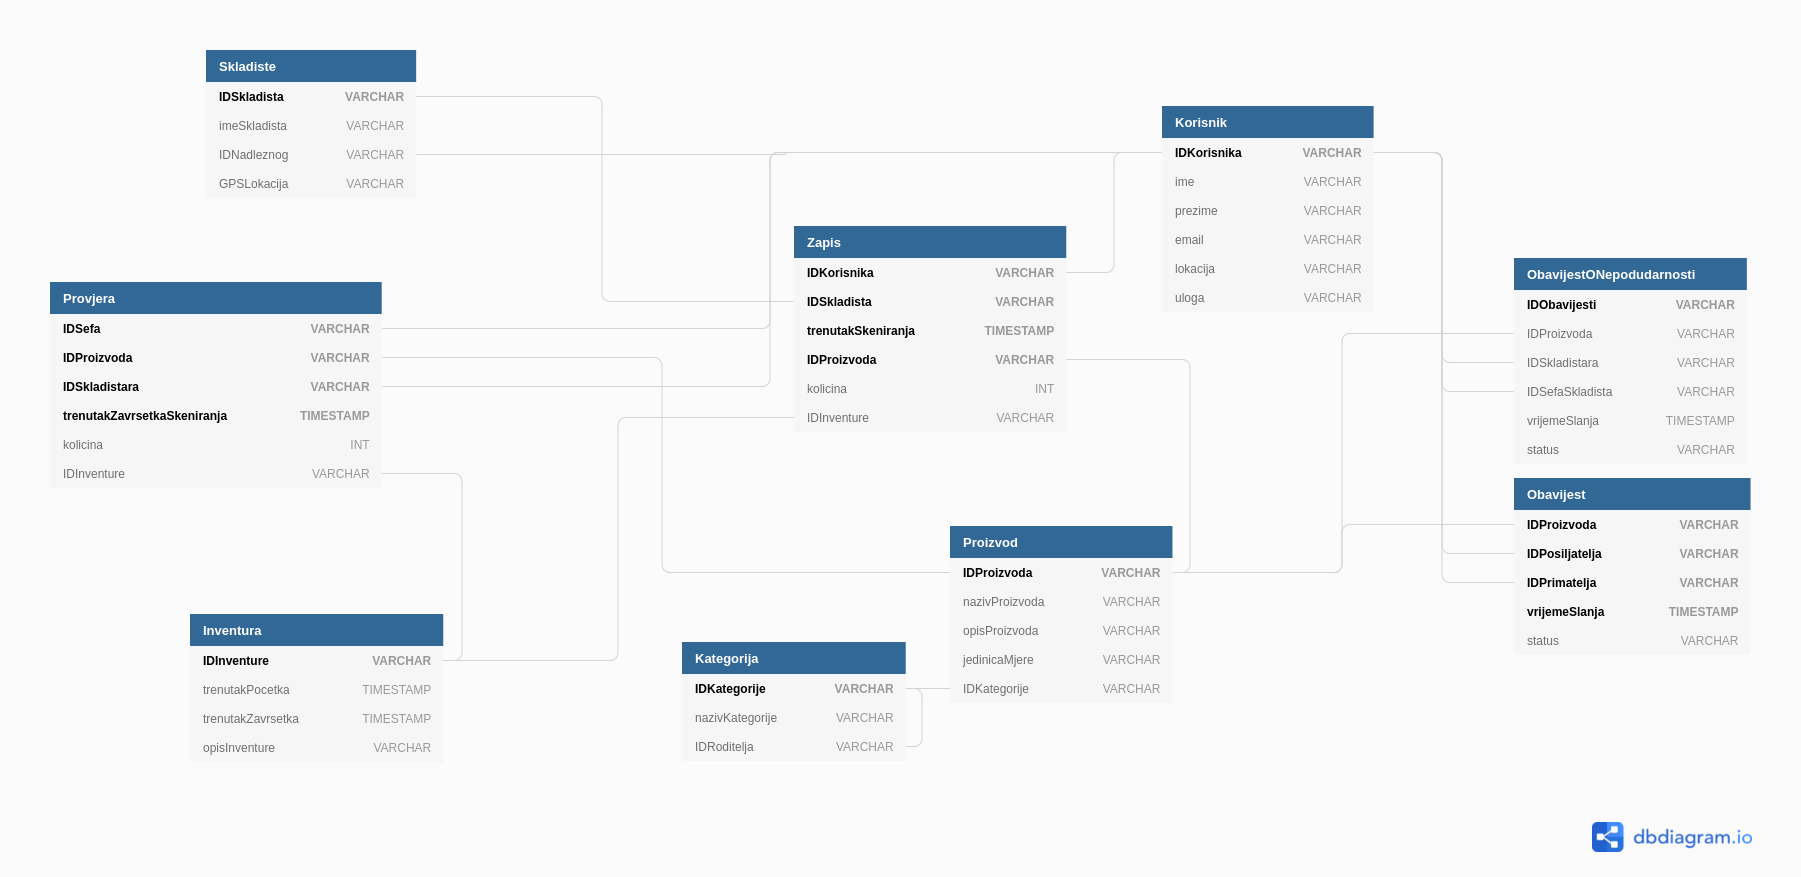
\includegraphics[scale=0.27]{"slike/ER_slika.png"}
					\caption{ER dijagram baze podataka}
					\label{Slika 4.1}
				\end{figure}
			
			\eject
			
			
		\section{Dijagram razreda}
			
			\begin{comment}
			\textbf{\textit{dio 1. revizije}}\\
			
			\textit{Prilikom prve predaje projekta, potrebno je priložiti potpuno razrađen dijagram razreda vezan uz \textbf{generičku funkcionalnost} sustava. Ostale funkcionalnosti trebaju biti idejno razrađene u dijagramu sa sljedećim komponentama: nazivi razreda, nazivi metoda i vrste pristupa metodama (npr. javni, zaštićeni), nazivi atributa razreda, veze i odnosi između razreda.}\\
			\end{comment}
			
			Na slikama 4.2 i 4.3 prikazani su razredi koji pripadaju backend dijelu aplikacije. Razredi sa slike 4.2 nasljeđuju razred Person i implementiraju dodatne potrebne metode. Razred Person sadrži još dodatno atribut role, koji je po tipu enumeracija Role. Slika 4.3 prikazuje odnose razreda koji se međusobno ne nasljeđuju.
			\begin{figure}[H]
				\centering
				\includegraphics[width=1.0\linewidth]{"slike/Class Diagram0"}
				\caption{Dijagram razreda - razredi koji nasljeđuju razred Person}
				\label{Slika 4.2}
			\end{figure}
			
			\begin{figure}[H]
				\centering
				\includegraphics[width=1.0\linewidth]{"slike/Class Diagram1"}
				\caption{Dijagram razreda - odnosi među klasama}
				\label{Slika 4.3}
			\end{figure}
			
			Svi razredi prikazani na slici 4.3 komuniciraju s bazom podataka kako bi dohvatili i spremili potrebne atribute. Razred Director ima najveće ovlasti. Nakon njega ide razred Manager, pa nakon njega Worker.
			
			\begin{comment}
			\textbf{\textit{dio 2. revizije}}\\			
			
			\textit{Prilikom druge predaje projekta dijagram razreda i opisi moraju odgovarati stvarnom stanju implementacije}
			\end{comment}
			
			
			\eject
		
		\section{Dijagram stanja}
			
			\begin{comment}
			
			\textbf{\textit{dio 2. revizije}}\\
			
			\textit{Potrebno je priložiti dijagram stanja i opisati ga. Dovoljan je jedan dijagram stanja koji prikazuje \textbf{značajan dio funkcionalnosti} sustava. Na primjer, stanja korisničkog sučelja i tijek korištenja neke ključne funkcionalnosti jesu značajan dio sustava, a registracija i prijava nisu. }
			
			\end{comment}
		
			\begin{figure}[H]
				\centering
				\includegraphics[width=1.0\linewidth]{"slike/Dijagram stanja"}
				\caption{Dijagram stanja - paljenje kamere i skeniranje artikala}
				\label{Slika 4.4}
			\end{figure}
		
			Slika 4.4 prikazuje dijagram stanja aplikacije prilikom pokretanja kamere. Prvi zadatak aplikacije je pokrenuti kameru na uređaju korisnika. Ukoliko pokretanje kamere nije moguće, dojavljuje se pogreška i izlazi se iz prozora. Ako je kamera uspješno pokrenuta, korisnik započinje skeniranje artikla. Najprije se dohvaćaju podaci o artiklu iz baze podataka i prikazuju se korisniku. Zatim, korisnik ažurira vrijednosti artikala te se, prilikom dovršetka rada, promjene spremaju u bazu podataka i kamera se gasi.
			
			\eject 
		
		
		\section{Dijagram aktivnosti}
			
			\begin{comment}
				\textbf{\textit{dio 2. revizije}}\\
				
				\textit{Potrebno je priložiti dijagram aktivnosti s pripadajućim opisom. Dijagram aktivnosti treba prikazivati značajan dio sustava.}
			\end{comment}
		
			\begin{figure}[H]
				\centering
				\includegraphics[width=1.0\linewidth]{"slike/Dijagram aktivnosti"}
				\caption{Dijagram aktivnosti - skeniranje artikla i komunikacija s bazom podataka}
				\label{Slika 4.5}
			\end{figure}
			
			Slika 4.5 prikazuje paljenje kamere i ažuriranje podataka o skeniranom artiklu u bazi podataka. Prvo se provjerava status kamere. Ukoliko se kamera nije uspjela pokrenuti, prekida se proces skeniranja artikla. Ako se kamera pokrenula, uspostavlja se veza s bazom podataka, kako bi korisnik mogao dohvatiti podatke o skeniranom artiklu. Ukoliko se veza s bazom podataka nije uspjela uspostaviti, prekida se proces skeniranja artikla. U suprotnom, baza podataka vraća podatke o traženom artiklu te se ti podaci prikazuju korisniku u obliku pop-up screena. Korisnik tu unosi nove vrijednosti, koje se u bazu podataka spremaju na dva načina: nakon isteka vremena od 5 sekundi ili kada korisnik pritisne gumb "Spremi". Korisnik također može prekinuti skeniranje artikla u bilo kojem trenutku, pritiskom bilo gdje na ekran uređaja, prilikom čega se odbacuju izmjene. Na kraju, ukoliko se podaci nisu uspjeli spremiti u bazu, gasi se skeniranje artikala. Ukoliko su podaci uspješno spremljeni, aplikacija završava normalno s radom i korisnik može započeti novo skeniranje artikla.
			
			\eject
			
		\section{Dijagram komponenti}
		
			\begin{comment}
				\textbf{\textit{dio 2. revizije}}\\
				
				\textit{Potrebno je priložiti dijagram komponenti s pripadajućim opisom. Dijagram komponenti treba prikazivati strukturu cijele aplikacije.}
			\end{comment}
		 	
		 	\begin{figure}[H]
		 		\centering
		 		\includegraphics[width=0.8\linewidth]{"slike/Dijagram komponenti"}
		 		\caption{Dijagram komponenti - struktura aplikacije}
		 		\label{Slika 4.6}
		 	\end{figure}
	 	
	 		Slika 4.6 prikazuje rad i komunikaciju između pojedinih komponenti aplikacije. Aplikacija je namijenjena za pokretanje na mobilnim uređajima, a pisana je u Flutteru. Podaci potrebni za rad aplikacije se dohvaćaju iz Firestore baze podataka.
			 
	\chapter{Implementacija i korisničko sučelje}
		
		
		\section{Korištene tehnologije i alati}
		
			Da bi postigli bolju komunikaciju te se bolje organizirali oko podjele zadataka koristili smo aplikacije Discord\footnote{\url{https://discord.com/}} i WhatsApp\footnote{\url{https://www.whatsapp.com/}}. Za izradu dokumentacije smo koristili TeXstudio\footnote{\url{https://www.texstudio.org/}} - integrirano okruženje za pisanje LaTex dokumenata, a za UML dijagrame smo koristili Astah Proffesional\footnote{\url{http://astah.net/editions/professional}}. Udaljeni repozitorij projekta dostupan je na web platformi Gitlab\footnote{\url{https://gitlab.com/}}.
			
			Kao razvojno okruženje koristili smo Visual Studio Code\footnote{\url{https://code.visualstudio.com/}} - uređivač izvornog koda koji je napravio Microsoft. VS Code ima ugrađeni sustav za upravljanje izvornim kodom Git\footnote{\url{https://git-scm.com/}} koji smo koristili u ovom projektu.
			
			Aplikacija je napravljena uz pomoć radnog okvira Flutter\footnote{\url{https://flutter.dev/multi-platform/mobile}} i programsog jezika Dart\footnote{\url{https://dart.dev/}}. Flutter je održavan od strane Google-a, a koristi se za razvoj aplikacija za različite sustave - najčešće za razvoj mobilnih aplikacija za android i IOS. Baza podataka se nalazi na poslužitelju Firebase\footnote{\url{https://firebase.google.com/}} koji je također nastao od strane Google-a. Firebase je software koji nudi razne usluge za lakšu i bržu izradu Android, IOS i web aplikacija.
			
			\eject 
		
	
		\section{Ispitivanje programskog rješenja}
	
			
			\subsection{Ispitivanje komponenti}
			
			Budući da je aplikacija napisana za Android uređaje koristeći Flutter, za testove je korišten implementirani paket \textit{flutter\textunderscore test: sdk: flutter} pomoću kojeg su napravljeni unit testovi aplikacije.
			
			Testiraju se razne funkcionalnosti dostupne na android uređaju, među kojima vrijedi izdvojiti testiranje stvaranja novog skladištara, stvaranje novog proizvoda, Unos novog zapisa skeniranja artikla, stvaranje nove grupe proizvoda, stvaranje nove inventure i obavijesti da proizvod ne postoji.
			
			Primjer testiranja:
			
			\begin{figure}[H]
				\centering
				\includegraphics[width=0.8\linewidth]{"slike/Test1"}
				\caption{Screenshot unit test koda (1)}
				\label{Slika 5.1}
			\end{figure}
			
			\begin{figure}[H]
				\centering
				\includegraphics[width=0.8\linewidth]{"slike/Test2"}
				\caption{Screenshot unit test koda (2)}
				\label{Slika 5.2}
			\end{figure}
			
			\begin{figure}[H]
				\centering
				\includegraphics[width=0.8\linewidth]{"slike/Test3"}
				\caption{Rezultati unit testiranja}
				\label{Slika 5.3}
			\end{figure}
			
			
			
			\subsection{Ispitivanje sustava}
			
			 Ispitivanje sustava je provedeno koristeći funkcionalnosti iz flutterovog paketa integration\textunderscore test kojeg je potrebno instalirati tako da se u pubspec.yaml file pod dev\textunderscore dependencies dodaju sljedeće linije\\
			
			 \begin{verbatim}
			 	integration_test:
			 		sdk: flutter
			 \end{verbatim}
		 	i u terminal unese naredba flutter pub get. Sav kod za ispitivanje sustava napisan je u programskom jeziku dart. Nad sustavom proveli smo sljedeća testiranja:
		 	
		 	Otvaranje pop up prozora nakon pritiska gumba za skeniranje:
		 	\begin{verbatim}
		 		testWidgets('Skeniraj i otvori pop up', (WidgetTester tester) async {
		 			app.main();
		 			await tester.pumpAndSettle();
		 			final Finder scan = find.byTooltip('scan');
		 			await tester.tap(scan);
		 			expect(find.byType(AlertDialog), findsOneWidget);
		 		});
		 	\end{verbatim}
	 		
	 		Otvaranje pop up prozora prilikom dodavanja novoga skladišta:
	 		\begin{verbatim}
	 			testWidgets('Otvaranje dialoga prilikom dodavanja skladišta', (WidgetTester tester) async {
	 				app.main();
	 				await tester.pumpAndSettle();
	 				final Finder addWarehouse = find.byTooltip('addWarehouse');
	 				await tester.tap(addWarehouse);
	 				expect(find.byType(AlertDialog), findsOneWidget);
	 			});
	 		\end{verbatim}
 			
 			Upisivanje podataka za prijavu:
 			\begin{verbatim}
 				testWidgets('Upisivanje podataka za prijavu', (WidgetTester tester) async {
 					app.main();
 					await tester.pumpAndSettle();
 					final Finder inputEmail = find.byKey(Key('email'));
 					final Finder inputPass = find.byKey(Key('inputPass'));
 					await tester.enterText(inputEmail, 'fb@gmail.com');
 					await tester.enterText(inputPass, '123456');
 					expect(find.text('fb@gmail.com'), findsOneWidget);
 					expect(find.text('123456'), findsOneWidget);
 				});
 			\end{verbatim}
 		
 			Upisivanje podataka za registraciju:
 			\begin{verbatim}
 				testWidgets('Upisivanje podataka za registraciju', (WidgetTester tester) async {
 					app.main();
 					await tester.pumpAndSettle();
 					final Finder inputName = find.byKey(Key('name'));
 					final Finder inputLastName = find.byKey(Key('lastName'));
 					final Finder inputEmail = find.byKey(Key('email'));
 					final Finder inputPass = find.byKey(Key('inputPass'));
 					await tester.enterText(inputName, 'Filip');
 					await tester.enterText(inputLastName, 'Begović');
 					await tester.enterText(inputEmail, 'fb@gmail.com');
 					await tester.enterText(inputPass, '123456');
 					expect(find.text('Filip'), findsOneWidget);
 					expect(find.text('Begović'), findsOneWidget);
 					expect(find.text('fb@gmail.com'), findsOneWidget);
 					expect(find.text('123456'), findsOneWidget);
 				});
 			\end{verbatim}
		
		\section{Dijagram razmještaja}
			
			Dijagram razmještaja opisuje topologiju sustava i usredotočen je na odnos sklopovskih i programskih dijelova. Na \textit{Firebase} platformi nalaze se tri glavna artefakta kojima upravljamo bazom podataka. Klijent preko aplikacije pristupa bazi podataka. Sustav je baziran na obliku "poslužiteljske arhitekture". Komunikacija između mobilnog uređaja  (skladištar, voditelj skladišta i direktora) i \textit{Firebase} odvija se preko SDK veze.
			
			\begin{figure}[H]
				\centering
				\includegraphics[width=0.8\linewidth]{"slike/Deployment Diagram"}
				\caption{Specifikacijski dijagram razmještaja}
				\label{Slika 5.4}
			\end{figure}
			
			\eject 
		
		\section{Upute za puštanje u pogon}
		
			Upute za puštanje u pogon napisane su za windows operacijski sustav. Za pokretanje aplikacije na vlastitom mobitelu potrebno je prvo napraviti \textit{google profil}, te preuzeti aplikaciju s google diska (\textbf{Ovdje dolazi link aplikacije}). Kada se cijela aplikacija preuzela u željenu mapu na računalu potrebno je instalirati Flutter.
			
			Prvo unesite link u vaš preglednik: \url{https://git-scm.com/download/win} te odaberite verziju koja odgovara vašem računalu (32-bit ili 64-bit). Nakon preuzimanja, pokrenite preuzeti \textit{.exe file} te pratite upute do kraja instalacije.
			
			Nakon toga unesite \url{https://docs.flutter.dev/get-started/install/windows} u vaš preglednik te provjerite je li vaše računalo zadovoljava potrebne specifikacije. Ispod podnaslova \textit{Get the Flutter SDK} pritisnite plavi gumb: \textit{flutter\textunderscore windows\textunderscore 2.8.1-stable.zip}. Nakon preuzimanja .zip mape te izvucite datoteke u mapu C:/src/.
			
			Potom je potrebno dodati PATH kako bi smo lakše koristili flutter kasnije. Pratite mape gdje ste instalirali flutter sve dok ne dođete do bit mape (najvjerojarnije putanja: C:/src/FlutterSDK/flutter/bin) te kopirajte tu putanju pošto će nam trebati poslije. U Windows tražilicu potrebno je upisati \textit{Control panel} te odabrati \textit{System}. S lijeve strane nalaziti će se popis opcija gdje je potrebno odabrati \textit{Additional settings}. Odaberite \textit{Edit enviroment variables for your account} te će vam se otvoriti prozor podijeljen na dva dijela. U gornjem prozoru nađite varijablu imenom \textit{Path}, pritisnite na nju te ispod pritisnite \textit{Edit}. S desne strane pritisnite \textit{New} te zalijepite kopiranu putanju do mape bin. Potom u odjeljku ispod nađite ponovno varijablu \textit{Path} te ponovite isti postupak kao i prethodno naveden. Pritisnite OK te izađite van.
			
			Provjerom uspješnosti instalacije \textit{fluttera} istovremeno ćete saznati je li određene potrebne datoteke nedostaju. U CMD-u napišite naredbu \textit{flutter doctor}. Povratna informacija će izbaciti kako nedostaje Android SDK, koji nam je sada nepotreban.
			
			Otvorite VS Code te u opciji \textit{Open Folder} otvorite mapu u kojoj se nalazi aplikacija. Odaberite opciju \textit{Extensions} te preuzmite i u VS Code \textit{Flutter} i \textit{Dart}.
			
			Nakon što je sve potrebno instalirano i aplikacija otvorena u VS Code, u \textit{Terminal} se može upisati naredba: flutter build apk --build-name=1.0.1 --build-number=2 koja pokreće \textit{build} aplikacije. Nakon što se proces završi u početnoj mapi projekta u \textit{File Explorer} pratite putanju: \textit{build/app/outputs/apk} te će datoteka pod nazivom apk-release.apk biti završna i primjenjiva aplikacija projekta. Za kraj je potrebno prebaciti apk datoteku na mobilni uređaj te pokrenuti instalaciju.
			
			
			\eject 
	\chapter{Zaključak i budući rad}
		
		 
		 Zadani zadatak naše grupe bio je razvoj rješenja problema vođenja inventure unutar više skladišta jedne kompanije, statistike greške skladištara koji vode inventuru i pomoću lokacije praćenje zaposlenika te kojim skladištima pripadaju. U razdoblju ovog semestra smo uspješno razvili aplikaciju te ostvarili zadani cilj. Provedba samog projekta odvijala se u dvije faze te smo unutar tima bili podijeljeni u dvije manje grupe zadužene za \textit{frontend} i \textit{backend} (podjela nije bila isključujuća te su članovi tima si međusobno kontinuirano pomagali radi bolje izvedbe i lakše komunikacije).
		 	
		 Prva faza razvoja aplikacije bila je okupljanje tima, dodjelu projektnog zadatka te praćenjem i dokumentiranjem zahtjeva određen obujam posla te inicijalna raspodjela poslova. Praćenjem daljnjih uputa te izradom obrazaca uporabe i dijagrama (sekvencijski dijagrami, dijagram razreda, model baze podataka (teže napravljen jer je baza podataka u Firebase-u, ali dovoljno da lakše shvatimo što je potrebno napraviti)) olakšana je raspodjela poslova među podtimovima i komunikacija među članovima jer smo se lakše mogli snaći u poslu koji je obavio drugi član. Izrada vizualnog dizajna aplikacije dodatno je olakšala razvoj u drugom ciklusu jer su podtimovi \textit{frontend} i \textit{backend} mogli brže raditi.
		 
		 Druga faza razvoja, programiranje zadane aplikacije, bila je puno zahtjevnija individualno zbog manjka iskustva u programiranju u zadanom razvojnom okruženju. Prije samog programiranja svaki član samostalno je proučio potrebne alate kako bi otprilike znali kako i izvedivost zahtjeva. Podjela poslova, iako u početku raspodijeljena individualno, većinom je tražila rad više članova koji su si međusobno pomagali i zajedno nalazili potrebna rješenja. Uz sam razvoj aplikacije bilo je potrebno daljnje praćenje UML dijagrama i održavanja projektne dokumentacije kako bi budući korisnici, a i članovi tima lakše snalazili u određenim dijelovima projekta. Kontinuirano praćenje i razvoja kostura aplikacije, prilagodba već napravljenih rješenja problema i intenzivna komunikacija članova omogućila nam je razvoj s minimalnim brojem grešaka i uštedu vremena u daljnjem programiranju.
		 
		 Za komunikaciju među članovima korištene su primarno dvije platforme: Whatsapp i Discord. Postojeće rješenje moguće je nastaviti razvijati i dalje koristeći mobilnu aplikaciju te čak i proširiti funkcionalnost dodatnim razvojem web aplikacije.
		 
		 Sudjelovanje na ovom projektu uvelike je koristilo svim članovima u razvoju vještina komuniciranja u većoj grupi, praćenje i pomaganje u radu više ljudi i učenjem u novim razvojnim okruženjima. Zadovoljni smo postignutim rješenjem koje je moguće nastaviti razvijati te primijeniti u stvarnom svijetu.
		
		\eject

\begin{comment}
	\textbf{\textit{dio 2. revizije}}\\
	
	\textit{U ovom poglavlju potrebno je napisati osvrt na vrijeme izrade projektnog zadatka, koji su tehnički izazovi prepoznati, jesu li riješeni ili kako bi mogli biti riješeni, koja su znanja stečena pri izradi projekta, koja bi znanja bila posebno potrebna za brže i kvalitetnije ostvarenje projekta i koje bi bile perspektive za nastavak rada u projektnoj grupi.}
	
	\textit{Potrebno je točno popisati funkcionalnosti koje nisu implementirane u ostvarenoj aplikaciji.}
\end{comment}
	\chapter*{Popis literature}
		\addcontentsline{toc}{chapter}{Popis literature}
	 	
 		\textbf{\textit{Kontinuirano osvježavanje}}
	
		\textit{Popisati sve reference i literaturu koja je pomogla pri ostvarivanju projekta.}
		
		
		\begin{enumerate}
			
			
			\item  Programsko inženjerstvo, FER ZEMRIS, \url{http://www.fer.hr/predmet/proinz}
			
			\item  I. Sommerville, "Software engineering", 8th ed, Addison Wesley, 2007.
			
			\item  T.C.Lethbridge, R.Langaniere, "Object-Oriented Software Engineering", 2nd ed. McGraw-Hill, 2005.
			
			\item  I. Marsic, Software engineering book``, Department of Electrical and Computer Engineering, Rutgers University, \url{http://www.ece.rutgers.edu/~marsic/books/SE}
			
			\item  The Unified Modeling Language, \url{https://www.uml-diagrams.org/}
			
			\item  Astah Community, \url{http://astah.net/editions/uml-new}
		\end{enumerate}
		
		 
	
	
	\begingroup
	\renewcommand*\listfigurename{Indeks slika i dijagrama}
	%\renewcommand*\listtablename{Indeks tablica}
	%\let\clearpage\relax
	\listoffigures
	%\vspace{10mm}
	%\listoftables
	\endgroup
	\addcontentsline{toc}{chapter}{Indeks slika i dijagrama}


	
	\eject 
		
	\chapter*{Dodatak: Prikaz aktivnosti grupe}
		\addcontentsline{toc}{chapter}{Dodatak: Prikaz aktivnosti grupe}
		
		\section*{Dnevnik sastajanja}
		
		\textbf{\textit{Kontinuirano osvježavanje}}\\
		
		 \textit{U ovom dijelu potrebno je redovito osvježavati dnevnik sastajanja prema predlošku.}
		
		\begin{packed_enum}
			\item  sastanak
			
			\item[] \begin{packed_item}
				\item Datum: 6. listopada 2021.
				\item Prisustvovali: K. Franić, E. Wachtler, T. Jukić, N. Anić, M. Bagarić, F. Begović
				\item Teme sastanka:
				\begin{packed_item}
					\item  Prvi sastanak - razrada opće ideje za aplikaciju
					\item  Dogovor oko mogućih tehnologija za razvoj aplikacije, razmjena iskustava i opće upoznavanje
				\end{packed_item}
			\end{packed_item}
			
			\item  sastanak
			\item[] \begin{packed_item}
				\item Datum: 13. listopada 2021.
				\item Prisustvovali: K. Franić, E. Wachtler, T. Jukić, N. Anić, M. Bagarić, F. Begović, B. Rebić-Taučer
				\item Teme sastanka:
				\begin{packed_item}
					\item  Prvi sastanak s asistentom - opće upute
				\end{packed_item}
			\end{packed_item}
		
			\item  sastanak
			\item[] \begin{packed_item}
				\item Datum: 20. listopada 2021.
				\item Prisustvovali: K. Franić, E. Wachtler, T. Jukić, N. Anić, M. Bagarić, F. Begović, B. Rebić-Taučer
				\item Teme sastanka:
				\begin{packed_item}
					\item  Pokušaj instaliranja i pokretanja programa za razvoj aplikacije
					\item  Kratko upoznavanje s Flutterom, članovi s iskustvom (Franić, Begović) objasnili su glavni koncept ostatku tima
					\item  FrontEnd tim predstavio je ideju za dizajn screenova
				\end{packed_item}
			\end{packed_item}
		
			\item  sastanak
			\item[] \begin{packed_item}
				\item Datum: 23. listopada 2021.
				\item Prisustvovali: E. Wachtler, T. Jukić, B. Rebić-Taučer
				\item Teme sastanka:
				\begin{packed_item}
					\item  Razvijanje osnovne ideje za BackEnd dio aplikacije
				\end{packed_item}
			\end{packed_item}
		
			\item  sastanak
			\item[] \begin{packed_item}
				\item Datum: 23. listopada 2021.
				\item Prisustvovali: F. Begović, M. Bagarić, N. Anić
				\item Teme sastanka:
				\begin{packed_item}
					\item  Dogovor oko izgleda i rasporeda elemenata na ekranima
				\end{packed_item}
			\end{packed_item}
		
			\item  sastanak
			\item[] \begin{packed_item}
				\item Datum: 28. listopada 2021.
				\item Prisustvovali: M. Bagarić, F. Begović
				\item Teme sastanka:
				\begin{packed_item}
					\item  Razgovor s asistentom i rješavanje pitanja u vezi zadataka aplikacije
					\item  Konzultacije oko funkcionalnih zahtjeva
				\end{packed_item}
			\end{packed_item}
		
			\item  sastanak
			\item[] \begin{packed_item}
				\item Datum: 29. listopada 2021.
				\item Prisustvovali: K. Franić, E. Wachtler, T. Jukić, N. Anić, M. Bagarić, F. Begović, B. Rebić-Taučer
				\item Teme sastanka:
				\begin{packed_item}
					\item  Prezentacija dosad napravljenog
					\item  Raspravljanje o pitanjima koja su se pojavila prilikom razvoja
				\end{packed_item}
			\end{packed_item}
		
			\item  sastanak
			\item[] \begin{packed_item}
				\item Datum: 04. studenoga 2021.
				\item Prisustvovali: K. Franić, E. Wachtler, T. Jukić, N. Anić, M. Bagarić, F. Begović, B. Rebić-Taučer
				\item Teme sastanka:
				\begin{packed_item}
					\item  Prezentacija dosad napravljenoga
					\item  Raspravljanje o pitanjima koja su se pojavila prilikom razvoja
				\end{packed_item}
			\end{packed_item}
		
			\item  sastanak
			\item[] \begin{packed_item}
				\item Datum: 07. studenoga 2021.
				\item Prisustvovali: K. Franić, N. Anić
				\item Teme sastanka:
				\begin{packed_item}
					\item  Ispravci pogrešaka za signup screen
					\item  Poboljšanje strukture koda
				\end{packed_item}
			\end{packed_item}
		
			\item  sastanak
			\item[] \begin{packed_item}
				\item Datum: 10. studenoga 2021.
				\item Prisustvovali: K. Franić, E. Wachtler, T. Jukić, B. Rebić-Taučer, N. Anić, F. Begović
				\item Teme sastanka:
				\begin{packed_item}
					\item  Rješavanje pitanja s asistentom koja su se pojavila prilikom razvoja aplikacije
				\end{packed_item}
			\end{packed_item}
		
			\item  sastanak
			\item[] \begin{packed_item}
				\item Datum: 12. studenoga 2021.
				\item Prisustvovali: K. Franić, E. Wachtler, T. Jukić, B. Rebić-Taučer
				\item Teme sastanka:
				\begin{packed_item}
					\item  Rješavanje pitanja u vezi komunikacije s bazom podataka
				\end{packed_item}
			\end{packed_item}
		
			\item  sastanak
			\item[] \begin{packed_item}
				\item Datum: 13. studenoga 2021.
				\item Prisustvovali: K. Franić, E. Wachtler
				\item Teme sastanka:
				\begin{packed_item}
					\item  Ispravljanje pogreške koja se javljala na nekim uređajima
				\end{packed_item}
			\end{packed_item}
		
			\item  sastanak
			\item[] \begin{packed_item}
				\item Datum: 14. studenoga 2021.
				\item Prisustvovali: K. Franić, E. Wachtler, T. Jukić, N. Anić, M. Bagarić, F. Begović, B. Rebić-Taučer
				\item Teme sastanka:
				\begin{packed_item}
					\item  Prezentacija dosad napravljenoga
					\item  Raspravljanje o pitanjima koja su se pojavila prilikom razvoja
					\item  Razrada ideje oko skeniranja artikala
				\end{packed_item}
			\end{packed_item}
		
			\item  sastanak
			\item[] \begin{packed_item}
				\item Datum: 18. studenoga 2021.
				\item Prisustvovali: K. Franić, E. Wachtler, T. Jukić, N. Anić, M. Bagarić, F. Begović, B. Rebić-Taučer
				\item Teme sastanka:
				\begin{packed_item}
					\item  Prezentacija dosad napravljenoga
					\item  Rješavanje pogrešaka za prvu predaju
					\item  Prezentacija dosad napravljenog asistentu
				\end{packed_item}
			\end{packed_item}
		
			\item sastanak
			\item[] \begin{packed_item}
				\item Datum: 18. prosinca 2021.
				\item Prisustvovali: K. Franić, E. Wachtler, T. Jukić, N. Anić, M. Bagarić, F. Begović, B. Rebić-Taučer
				\item Teme sastanka:
				\begin{packed_item}
					\item  Izrada aplikacije za prvu demonstraciju
					\item  Dodavanje potrebnih funkcionalnosti za komunikaciju s bazom podataka
				\end{packed_item}
			\end{packed_item}
		
			\item sastanak
			\item[] \begin{packed_item}
				\item Datum: 19. prosinca 2021.
				\item Prisustvovali: K. Franić, E. Wachtler, T. Jukić, N. Anić, M. Bagarić, F. Begović, B. Rebić-Taučer
				\item Teme sastanka:
				\begin{packed_item}
					\item  Izrada aplikacije za prvu demonstraciju
					\item  Implementacija dohvaćanja lokacije
					\item  Implementacija skeniranja artikala
				\end{packed_item}
			\end{packed_item}
		
			\item sastanak
			\item[] \begin{packed_item}
				\item Datum: 9. siječnja 2022.
				\item Prisustvovali: K. Franić, E. Wachtler, T. Jukić, F. Begović
				\item Teme sastanka:
				\begin{packed_item}
					\item  Izrada statistike za skladištara
					\item  Popravak rada aplikacije prilikom skeniranja
					\item  Popravak dohvata lokacije
				\end{packed_item}
			\end{packed_item}
		
			\item sastanak
			\item[] \begin{packed_item}
				\item Datum: 11. siječnja 2022.
				\item Prisustvovali: K. Franić, E. Wachtler, T. Jukić, F. Begović
				\item Teme sastanka:
				\begin{packed_item}
					\item  Popravak statistike za skladištara
					\item  Ispravci pogrešaka u radu aplikacije
					\item  Raspodjela daljnjih poslova
				\end{packed_item}
			\end{packed_item}
			
			%
			
		\end{packed_enum}
		
		\eject
		\section*{Tablica aktivnosti}
		
			\textbf{\textit{Kontinuirano osvježavanje}}\\
			
			 \textit{Napomena: Doprinose u aktivnostima treba navesti u satima po članovima grupe po aktivnosti.}

			\begin{longtblr}[
					label=none,
				]{
					vlines,hlines,
					width = \textwidth,
					colspec={X[7, l]X[1, c]X[1, c]X[1, c]X[1, c]X[1, c]X[1, c]X[1, c]}, 
					vline{1} = {1}{text=\clap{}},
					hline{1} = {1}{text=\clap{}},
					rowhead = 1,
				} 
				\multicolumn{1}{c|}{} & \multicolumn{1}{c|}{\rotatebox{90}{\textbf{Elena Wachtler}}} & \multicolumn{1}{c|}{\rotatebox{90}{\textbf{Karlo Franić}}} &	\multicolumn{1}{c|}{\rotatebox{90}{\textbf{Filip Begović}}} & \multicolumn{1}{c|}{\rotatebox{90}{\textbf{Nina Anić}}} &	\multicolumn{1}{c|}{\rotatebox{90}{\textbf{Marko Bagarić}}} & \multicolumn{1}{c|}{\rotatebox{90}{\textbf{Borna Rebić-Taučer}}} &	\multicolumn{1}{c|}{\rotatebox{90}{\textbf{Tin Jukić}}} \\  
				Upravljanje projektom 		& 20 & 10  & 3  &  &  &  & \\ 
				Opis projektnog zadatka 	& 1 &  & 12 & 6 & 6  & 3 & \\ 
				
				Funkcionalni zahtjevi       &  & 2 & 5 & 13 & 13 & 7 &  \\ 
				Opis pojedinih obrazaca 	& 2 &  & 8 & 15 & 3  &  &  \\ 
				Dijagram obrazaca 			&  &  & 6 &  &  & 2 &  \\ 
				Sekvencijski dijagrami 		&  &  & 5 &  &  &  & 3 \\ 
				Opis ostalih zahtjeva 		&  &  & 1 & 5 & 1 &  &  \\ 

				Arhitektura i dizajn sustava	& 8 & 8 & 9 & 8 & 8 & 5 & 5  \\ 
				Baza podataka				& 10 & 10 &  &  &  & 5 & 5  \\ 
				Dijagram razreda 			&  &  &  &  &  &  &  10 \\ 
				Dijagram stanja				&  &  &  &  &  &  & 2 \\ 
				Dijagram aktivnosti 		&  &  &  &  &  &  & 3 \\ 
				Dijagram komponenti			&  &  &  &  &  &  & 2 \\ 
				Korištene tehnologije i alati 		& 4 & 4 & 3 & 3 & 5 & 5 & 5 \\ 
				Ispitivanje programskog rješenja 	& 2 & 2 & 25 & 15 & 27 & 10 & 7  \\ 
				Dijagram razmještaja			&  &  &  &  &  & 2 &  \\ 
				Upute za puštanje u pogon 		&  &  &  &  & 5 & 2 &  \\  
				Dnevnik sastajanja 			&  &  &  &  &  &  & 7 \\ 
				Zaključak i budući rad 		&  &  &  &  & 6 &  &  \\  
				Popis literature 			&  &  &  &  &  & 2 &  \\  
				&  &  &  &  &  &  &  \\ \hline 
				\textit{front end} 				&  & 12 & 47 & 45 & 25 & 5 &  \\  
				\textit{izrada baze podataka} 		 			& 5 & 19 &  &  &  & 5 & 5 &\\  
				\textit{spajanje s bazom podataka} 							& 20 & 10 & 7 &  &  & 5 & 5 \\ 
				\textit{back end} 							& 49 & 55 &  &  &  & 40 & 40 \\  \hline
				 \textbf{ukupno sati}							& 121 & 132 & 131 & 110 & 99 & 98 & 99 \\ 
			\end{longtblr}
					
					
		\eject
		\section*{Dijagrami pregleda promjena}
		
		\begin{figure}[H]
			\centering
			\includegraphics[width=1.0\linewidth]{"slike/contributors_master"}
			\caption{Dijagram pregleda promjena 1}
			\label{Slika 6.1}
		\end{figure}
	
		\begin{figure}[H]
			\centering
			\includegraphics[width=1.0\linewidth]{"slike/contributors_auth"}
			\caption{Dijagram pregleda promjena 2}
			\label{Slika 6.2}
		\end{figure}
	
		\begin{figure}[H]
			\centering
			\includegraphics[width=1.0\linewidth]{"slike/contributors_devdoc"}
			\caption{Dijagram pregleda promjena 3}
			\label{Slika 6.3}
		\end{figure}
	
		\begin{figure}[H]
			\centering
			\includegraphics[width=1.0\linewidth]{"slike/contributors_scan"}
			\caption{Dijagram pregleda promjena 4}
			\label{Slika 6.4}
		\end{figure}
	
		\begin{figure}[H]
			\centering
			\includegraphics[width=1.0\linewidth]{"slike/contributors_scan2"}
			\caption{Dijagram pregleda promjena 5}
			\label{Slika 6.5}
		\end{figure}
	


\end{document} %naredbe i tekst nakon ove naredbe ne ulaze u izgrađen dokument 


